\documentclass[12pt,a4paper,openany,oneside]{book}

% 格式控制
%------------------------------------------------------------------------------%
%                                                                              %
%   LaTeX Template for Bachlor Thesis of Northwestern Polytechnical University %
%   Environment Config: TeXLive 2017                                           %
%   * XeTeX 3.14159265-2.6-0.99998 (TeX Live 2017/W32TeX)                      %
%   * BibTeX 0.99d (TeX Live 2017/W32TeX)                                      %
%   Version: 1.5.0.0426                                                        %
%                                                                              %
%------------------------------------------------------------------------------%
%   Copyright by NWPU Metaphysics Office, GPLv3-LICENSE                        %
%------------------------------------------------------------------------------%


%---------------------------------纸张大小设置---------------------------------%
\usepackage{geometry}
% 普通A4格式缩进
% \geometry{left=2.5cm,right=2.5cm,top=2.5cm,bottom=2.5cm}
% 论文标准缩进
\geometry{left=1.25in,right=1.25in,top=1in,bottom=1.5in}
%------------------------------------------------------------------------------%


%----------------------------------必要库支持----------------------------------%
\usepackage{xcolor}
\usepackage{tikz}
\usepackage{layouts}
\usepackage[numbers,sort&compress]{natbib}
\usepackage{clrscode}
\usepackage{gensymb}
\usepackage[final]{pdfpages}
%------------------------------------------------------------------------------%


%--------------------------------设置标题与目录--------------------------------%
\usepackage[sf]{titlesec}
\usepackage{titletoc}
%------------------------------------------------------------------------------%


%--------------------------------添加书签超链接--------------------------------%
\usepackage[unicode=true,colorlinks=false,pdfborder={0 0 0}]{hyperref}
% 在此处修改打开文件操作
\hypersetup{
    bookmarks=true,         % show bookmarks bar?
    pdftoolbar=true,        % show Acrobat’s toolbar?
    pdfmenubar=true,        % show Acrobat’s menu?
    pdffitwindow=true,      % window fit to page when opened
    pdfstartview={FitH},    % fits the width of the page to the window
    pdfnewwindow=true,      % links in new PDF window
}
% 在此处添加文章基础信息
\hypersetup{
    pdftitle={title},
    pdfauthor={author},
    pdfsubject={subject},
    pdfcreator={creator},
    pdfproducer={producer},
    pdfkeywords={key1  key2  key3}
}
%------------------------------------------------------------------------------%


%---------------------------------设置字体大小---------------------------------%
\usepackage{type1cm}
% 字号与行距,统一前缀s(a.k.a size)
\newcommand{\sChuhao}{\fontsize{42pt}{63pt}\selectfont}                 % 初号, 1.5倍
\newcommand{\sYihao}{\fontsize{26pt}{36pt}\selectfont}                  % 一号, 1.4倍
\newcommand{\sErhao}{\fontsize{22pt}{28pt}\selectfont}                  % 二号, 1.25倍
\newcommand{\sXiaoer}{\fontsize{18pt}{18pt}\selectfont}                 % 小二, 单倍
\newcommand{\sSanhao}{\fontsize{16pt}{24pt}\selectfont}                 % 三号, 1.5倍
\newcommand{\sXiaosan}{\fontsize{15pt}{22pt}\selectfont}                % 小三, 1.5倍
\newcommand{\sSihao}{\fontsize{14pt}{21pt}\selectfont}                  % 四号, 1.5倍
\newcommand{\sHalfXiaosi}{\fontsize{12.5pt}{16.25pt}\selectfont}        % 半小四, 1.25倍
\newcommand{\sLargeHalfXiaosi}{\fontsize{13pt}{19pt}\selectfont}        % 半小四, 1.5倍
\newcommand{\sXiaosi}{\fontsize{12pt}{14.4pt}\selectfont}               % 小四, 1.25倍
\newcommand{\sLargeWuhao}{\fontsize{11pt}{11pt}\selectfont}             % 大五, 单倍
\newcommand{\sWuhao}{\fontsize{10.5pt}{10.5pt}\selectfont}              % 五号, 单倍
\newcommand{\sXiaowu}{\fontsize{9pt}{9pt}\selectfont}                   % 小五, 单倍
%------------------------------------------------------------------------------%


%---------------------------------设置中文字体---------------------------------%
\usepackage{fontspec}
\usepackage[SlantFont,BoldFont,CJKchecksingle]{xeCJK}
\usepackage{CJKnumb}
% 使用 Adobe 字体
\newcommand\adobeSog{Adobe Song Std}
\newcommand\adobeHei{Adobe Heiti Std}
\newcommand\adobeKai{Adobe Kaiti Std}
\newcommand\adobeFag{Adobe Fangsong Std}
\newcommand\codeFont{Consolas}
% 设置字体
\defaultfontfeatures{Mapping=tex-text}
\setCJKmainfont[ItalicFont=\adobeKai, BoldFont=\adobeHei]{\adobeSog}
\setCJKsansfont[ItalicFont=\adobeKai, BoldFont=\adobeHei]{\adobeSog}
\setCJKmonofont{\codeFont}
\setmonofont{\codeFont}
% 设置字体族
\setCJKfamilyfont{song}{\adobeSog}      % 宋体
\setCJKfamilyfont{hei}{\adobeHei}       % 黑体
\setCJKfamilyfont{kai}{\adobeKai}       % 楷体
\setCJKfamilyfont{fang}{\adobeFag}      % 仿宋体
% 用于页眉学校名,特殊字体,powerby https://github.com/ecomfe/fonteditor
\setCJKfamilyfont{nwpu}{nwpuname}
% 新建字体命令,统一前缀f(a.k.a font)
\newcommand{\fSong}{\CJKfamily{song}}
\newcommand{\fHei}{\CJKfamily{hei}}
\newcommand{\fFang}{\CJKfamily{fang}}
\newcommand{\fKai}{\CJKfamily{kai}}
\newcommand{\fNWPU}{\CJKfamily{nwpu}}
%------------------------------------------------------------------------------%


%------------------------------添加插图与表格控制------------------------------%
\usepackage{graphicx}
\usepackage[font=small,labelsep=quad]{caption}
\usepackage{wrapfig}
\usepackage{multirow,makecell}
\usepackage{longtable}
\usepackage{booktabs}
\usepackage{tabularx}
\usepackage{setspace}
\captionsetup[table]{labelfont=bf,textfont=bf}
%------------------------------------------------------------------------------%


%---------------------------------添加列表控制---------------------------------%
\usepackage{enumerate}
\usepackage{enumitem}
%------------------------------------------------------------------------------%


%---------------------------------设置引用格式---------------------------------%
\renewcommand\figureautorefname{图}
\renewcommand\tableautorefname{表}
\renewcommand\equationautorefname{式}
\newcommand\myreference[1]{[\ref{#1}]}
\newcommand\eqrefe[1]{式(\ref{#1})}
% 增加 \ucite 命令使显示的引用为上标形式
\newcommand{\ucite}[1]{$^{\mbox{\scriptsize \cite{#1}}}$}
\renewcommand\arraystretch{1.4}
\renewcommand\theequation{\thesection.\arabic{equation}}
\renewcommand{\thefigure}{\thechapter-\arabic{figure}}
\renewcommand{\thetable}{\thechapter-\arabic{table}}
%------------------------------------------------------------------------------%


%--------------------------------设置定理类环境--------------------------------%
\usepackage[amsthm,thmmarks]{ntheorem}
\newtheorem{myexample}{例}
\newtheorem{thm}{定理}
%------------------------------------------------------------------------------%


%--------------------------设置中文段落缩进与正文版式--------------------------%
\XeTeXlinebreaklocale "zh"                      % 使用中文的换行风格
\XeTeXlinebreakskip = 0pt plus 1pt              % 调整换行逻辑的弹性大小
\usepackage{indentfirst}                        % 段首空格设置
\setlength{\parindent}{26pt}                    % 段首空格长度
\setlength{\parskip}{3pt plus 1pt minus 1pt}    % 段落间距
\renewcommand{\baselinestretch}{1.25}           % 行距
%------------------------------------------------------------------------------%


%----------------------------设置段落标题与目录格式----------------------------%
\setcounter{secnumdepth}{3}
\setcounter{tocdepth}{2}

\newcommand\chapterID[1]{第\CJKnumber{#1}章}
\renewcommand{\chaptername}{第~\CJKnumber{\thechapter}~章}
\renewcommand{\figurename}{图}
\renewcommand{\tablename}{表}
\renewcommand{\bibname}{参考文献}
\renewcommand{\contentsname}{目~录}
\newcommand{\keywords}[1]{\\ \\ \textbf{关~键~词}:#1}


\titleformat{\chapter}[hang]{\normalfont\sSanhao\filcenter\fHei\bf}%
{\sSanhao{\chaptertitlename}}{20pt}{\sSanhao}
\titleformat{\section}[hang]{\fHei \bf \sXiaosan}%
{\sXiaosan \thesection}{0.5em}{}{}
\titleformat{\subsection}[hang]{\fHei \bf \sLargeHalfXiaosi}%
{\sLargeHalfXiaosi \thesubsection}{0.5em}{}{}
\titleformat{\subsubsection}[hang]{\fHei \bf}%
{(\arabic{subsubsection})}{0.5em}{}{}   % 小标题式的subsubsection:(4) 标题

% 缩小正文中各级标题之间的缩进
\titlespacing{\chapter}{0pt}{-3ex plus .1ex minus .2ex}{0.25em}
\titlespacing{\section}{0pt}{-0.2em}{0em}
\titlespacing{\subsection}{0pt}{0.5em}{0em}
\titlespacing{\subsubsection}{0pt}{0.25em}{0pt}

% 定义目录中各级标题之间的格式以及缩进
\dottedcontents{section}[1.16cm]{}{1.8em}{5pt}
\dottedcontents{subsection}[2.00cm]{}{2.7em}{5pt}
\dottedcontents{subsubsection}[2.86cm]{}{3.4em}{5pt}
\titlecontents{chapter}[0pt]{\fHei\vspace{0.5em}}%
{\contentsmargin{0pt}\fHei\makebox[0pt][l]{\chapterID{\thecontentslabel}}\hspace{3.8em}}%
{\contentsmargin{0pt}\fHei}%
{\titlerule*[.5pc]{.}\contentspage}[\vspace{0em}]
%------------------------------------------------------------------------------%


%---------------------------------设置页眉页脚---------------------------------%
\usepackage{fancyhdr}
\usepackage{fancyref}
%\addtolength{\headsep}{-0.1cm}          %页眉位置
%\addtolength{\footskip}{-0.1cm}         %页脚位置
\addtolength{\topmargin}{0.5cm}
\newcommand{\makeheadrule}{
    \makebox[0pt][l]{\rule[.7\baselineskip]{\headwidth}{0.8pt}}
    \vskip-.8\baselineskip
}
\makeatletter
\renewcommand{\headrule}{%
    {\if@fancyplain\let\headrulewidth\plainheadrulewidth\fi\makeheadrule}}
\pagestyle{fancyplain}
\fancyhf{}
\fancyfoot[C,C]{\sWuhao-~\thepage~-}
% 后续文字可以自行修改
\chead{\sSanhao\raisebox{0.04cm}%
    { \fNWPU 西北工业大学} \fSong{{\textbf{本科毕业设计论文} }}}
%------------------------------------------------------------------------------%


%----------------------------------其他补充设置--------------------------------%
% 重置列表环境的间隔
% \let\orig@Itemize =\itemize
% \let\orig@Enumerate =\enumerate
% \let\orig@Description =\description

% \def\Myspacing{
%     \itemsep=1.5ex \topsep=-0.5ex \partopsep=0pt \parskip=0pt \parsep=0.5ex
% }

% \def\newitemsep{
%     \renewenvironment{itemize}{\orig@Itemize\Myspacing}{\endlist}
%     \renewenvironment{enumerate}{\orig@Enumerate\Myspacing}{\endlist}
%     \renewenvironment{description}{\orig@Description\Myspacing}{\endlist}
% }

% \def\olditemsep{
%     \renewenvironment{itemize}{\orig@Itemize}{\endlist}
%     \renewenvironment{enumerate}{\orig@Enumerate}{\endlist}
%     \renewenvironment{description}{\orig@Description}{\endlist}
% }

% \newitemsep
% 下划线
\newcommand\dlmu@underline[2][5cm]%
{\hskip1pt\underline{\hb@xt@ #1{\hss#2\hss}}\hskip3pt}
\let\coverunderline\dlmu@underline
%------------------------------------------------------------------------------%


%----------------------------------添加代码控制--------------------------------%
\usepackage{listings}
\lstset{
    basicstyle=\footnotesize\ttfamily,
    numbers=left,
    numberstyle=\tiny,
    numbersep=5pt,
    tabsize=4,
    extendedchars=true,
    breaklines=true,
    keywordstyle=\color{blue}\bfseries,
    numberstyle=\color{purple},
    commentstyle=\color[rgb]{0, 0.4, 0}\bfseries,
    stringstyle=\color{violet}\ttfamily\bfseries,
    rulesepcolor=\color{red!20!green!20!blue!20},
    showspaces=false,
    showtabs=false,
    frame=shadowbox,
    framexrightmargin=5pt,
    framexbottommargin=4pt,
    showstringspaces=false,
    escapeinside=`', %逃逸字符(1左面的键),用于显示中文
}
\renewcommand{\lstlistingname}{CODE}
\lstloadlanguages{% Check Dokumentation for further languages, page 12
    Pascal, C++, Java, Ruby, Python, Matlab, R, Haskell
}
%------------------------------------------------------------------------------%

\endinput
% 这是简单的 thesis(book) 的导言区设置,不能单独编译。

\DeclareMathSizes{12}{20}{14}{10}

% 非格式控制插件
% \usepackage{math-symbols}
\usepackage{plug-ins/math-symbols}
\input{plug-ins/aerocoeffs}

\usepackage{subfigure}
\usepackage{multirow}
\usepackage{url}
\usepackage[ruled,linesnumbered,algochapter]{algorithm2e}

% listset --- start
\lstset{
language=C++,
basicstyle=\small\ttfamily,
numbers=left,
numbersep=5pt,
xleftmargin=20pt,
frame=tb,
framexleftmargin=20pt,
frame=shadowbox
}

\renewcommand*\thelstnumber{\arabic{lstnumber}:}

\DeclareCaptionFormat{mylst}{\hrule#1#2#3}
\captionsetup[lstlisting]{format=mylst,labelfont=bf,singlelinecheck=off,labelsep=space}

% listset --- end


% 插图目录
\graphicspath{{figures/}}

% 仅用于测试
\usepackage{blindtext}

\title{\textsf{基于华为鲲鹏920的SpTRSV算法优化}}
\author{{\kai 严愉程}}
\date{June 1, 2021}

\begin{document}

\sloppy

\pagenumbering{Roman}

% 封皮
\frontmatter
% 本科毕业设计论文模板
% 封皮
\begin{titlepage}
    \voffset 2.7cm
    \begin{center}
        \begin{center}
            \begin{minipage}[c]{2.64cm}
                \centering
                \resizebox{!}{0.9cm}{ \parbox{0.54cm}{ \input{settings/logo} } }
                \end{minipage}
                \hskip 0.8cm
                \begin{minipage}[c]{8cm}
                \fontsize{33}{33}\fNWPU 西北工业大学
            \end{minipage}
        \end{center}
        \vskip 0.7cm
        \sChuhao\fSong {\bfseries 本科毕业设计论文}
        \vskip 5cm
        {
        \sSanhao\fHei 题~~目 \hspace{0.2cm}\coverunderline[12.5cm]{基于华为鲲鹏920的SpTRSV算法优化}
        }
        \vskip 2cm
        {
            \sSihao\fSong 专业名称\coverunderline[5.5cm]{计算机科学与技术}
            \vskip 0.7cm
            \sSihao\fSong 学生姓名\coverunderline[5.5cm]{严愉程}
            \vskip 0.7cm
            \sSihao\fSong 指导教师\coverunderline[5.5cm]{王云岚}
            \vskip 0.7cm
            \sSihao\fSong 完成时间\coverunderline[5.5cm]{2021年6月1日}
            \vfill
        }
    \end{center}
\end{titlepage}
\fSong \normalsize

\endinput
% 这是封面排版文件,不能单独编译。

\setcounter{page}{1}
\renewcommand{\baselinestretch}{1.25}

% 中文摘要
\renewcommand{\baselinestretch}{1.5}
\fontsize{12pt}{13pt}\selectfont

\chapter[摘要]{摘~~~~要}
\markboth{中~文~摘~要}{中~文~摘~要}

稀疏下三角矩阵求解器(sparse triangular solver,SpTRSV),是数值计算中的一个重要的方法,在科学计算中有着广泛的应用。由于其离散的数据访存、任务之间存在着很强的依赖、需要细粒度的同步、任务之间负载不均衡等特点,在现代多核系统中,如何提升SpTRSV算法的并行度与扩展性,仍然是一个挑战性的课题。

华为鲲鹏920处理器基于ARMv8架构,最多拥有64个核心,支持ARM NEON 128bits浮点运算。华为鲲鹏系统支持NUMA内存架构,实现最多4个920互联,最高支持256个计算核心。

本文基于华为鲲鹏920芯片,进行稀疏下三角矩阵求解算法的设计与优化。

主要工作包括:% TODO:以下四点都要详细说明
\vspace{-10pt}
\begin{enumerate}
    \item 设计并实现了一套高效的稀疏下三角矩阵求解算法。与传统基于level-sets方法不同的是,该算法并没有采用构造任务依赖图(TDG)大幅减少了矩阵预处理的时间,使用原子操作以及自旋等待在运行时维护任务顺序。根据测试该算法相比于串行方法能够获得约2倍以上加速比, 并且在一些稀疏矩阵中能够取得比基于level-sets算法更好的性能提升。
    \item 针对华为鲲鹏920处理器众核体系结构以及ARMv8架构的特点进行了优化。在原有算法的基础上通过结合体系结构的优化(例如:消除为伪共享、使用ARMv8原子指令、CPU松弛等技术)能够进一步获得约10\%的性能提升。
    \item 采用ARM NEON指令,对向量乘法部分进行了SIMD的优化。对于float数据类型,进行了SIMD指令的优化,执行一条NEON乘法指令,相当于进行了四次乘法运算。
    \item 结合处理器NUMA架构的特性,对于规模较小的矩阵将任务绑定在单一的节点上,通过减少结点间的通信延迟,进行性能的优化。对于规模较大的矩阵,分配矩阵数据到不同节点上,通过充分利用内存带宽和核心数量,能够获得相比于单NUMA结点约15\%的性能提升。
\end{enumerate}
\vspace{-10pt}

\vspace{1em}
\noindent {\fHei 关键词:} \quad 稀疏下三角矩阵求解器, 鲲鹏920, 众核优化, 并行算法

\clearpage
\endinput

% 英文摘要
\renewcommand{\baselinestretch}{1.5}
\fontsize{12pt}{13pt}\selectfont

\chapter[ABSTRACT]{Abstract}
\markboth{英~文~摘~要}{英~文~摘~要}

The sparse triangular solve kernel(sparse triangular solver,SpTRSV), is an important building block for a number of numerical linear algebra routines. It is commonly considered challenging to parallelize and scale even on a moderate number of cores. This challenge is due to the fact that triangular solver typically has strong dependencies between tasks which rely on fine grained synchronization, frequent discrete memory access, and load embalances between tasks.

Huawei Kunpeng920 CPU is an ARMv8-based server CPU with up to 64 cores, supporting ARM NEON 128-bit SIMD instruction set and NUMA architecture with at most 4 nodes conected.

The main work of this article includes:
\vspace{-12pt}
\begin{enumerate} \setlength{\itemsep}{0pt}
    \item Design and implement an efficient sparse matrix triangular solve algorithm. Different with triditional level-sets based SpTRSV routine, without constructing task denpendence graph(TDG), our algorithm has greatly reduced the time cost of preprocessing stage. Instead, we use atomic operation and spin-wait to maintain the sequential between tasks. And our alogrithm is roughly 2 times faster than serial routine and better performance than level-sets based algorithm in some cases.
    \item Optimizing for Huawei Kunpeng920 and ARMv8 architecture.We have adopted several tricks related to the architecture of kunpeng920(e.g., eliminating false sharing, using ARMv8 new atomic instruction and cpu relax), achieved roughly 10\% further performance improvement.
    \item Utilizing ARM NEON 128bits SIMD instruction set to speed up the vector multiplication. As for the data type of float32, one NEON multiplication instruction is equal to 4 triditional multiplication instructions.
    \item Our alogrithm takes NUMA feature into consideration. For small matrix, we restrict all tasks in single node to avoid communication latency. And for large matrix, we allocate a copy of matrix data to every node, by utilizing larger bandwidth and more number of cores, our alogrithm running on multi-node has achieved 15\% performance boost than running on single node.
\end{enumerate}
\vspace{-12pt}


\vspace{1em}
\noindent {\textbf{Key Words:}} \quad SpTRSV, Kunpeng920, Multi-core Optimization, Parallel Algorithm

\clearpage
\endinput

\renewcommand{\baselinestretch}{1.25}
\fontsize{12pt}{12pt}\selectfont
\phantomsection
\addcontentsline{toc}{chapter}{\fHei 目录}
\tableofcontents
\clearpage

\mainmatter

\renewcommand{\baselinestretch}{1.25}
\sHalfXiaosi\fSong

% 正文内容
\chapter{绪论}
\section{课题背景}

稀疏下三角矩阵求解(Sparse Triangular Solve, SpTRSV)并行算法是很多数值计算方法的重要组成部分,比如用直接法求解稀疏矩阵的线性方程组\cite{davis2006direct},迭代法求解稀疏矩阵的预条件子\cite{elman1982iterative},以及最小二乘法的求解\cite{saad2003iterative},是现代科学计算中一个广泛使用的计算核心,在数值模拟计算中,通常会使用迭代法或直接法求解大规模稀疏线性方程组,而SpTRSV的效率直接影响了线性方程组的求解效率,故提高SpTRSV算法的性能至关重要。

相比于稠密下三角举证解法器\cite{hogg2013fast}或者其他稀疏矩阵计算方法,例如稀疏矩阵转置\cite{wang2016parallel},稀疏矩阵向量乘法\cite{liu2015csr5}\cite{liu2015speculative},和稀疏矩阵乘法\cite{liu2015framework},SpTRSV频繁且离散的数据访存、任务之间存在着很强的依赖、需要细粒度的同步、任务之间负载不均衡等特点使得并行优化更加难以进行。

SpTRSV算法主要是从方程组$Lx=b$中求解未知数向量$ x $,其中$ L $是下三角矩阵,且对角线上的元素都不为0。要计算其中的一个未知数$x_k$,需要先计算出其前置未知数$x_0$, \dots, $x_{k-1}$ 中的一个子集。这些任务间的依赖关系,将SpTRSV的计算转换成了一个任务依赖图的计算(Task Dependent Graph,TDG),并且这个TDG是一张有方无环图(Directed Acyclic Graph)。

华为作为鲲鹏计算产业的成员,聚焦于发展华为鲲鹏+昇腾双引擎芯片族,通过“硬件开放、软件开源、使能合作伙伴”来推动计算产业的发展。华为鲲鹏920处理器兼容了ARMv8架构。最多拥有64核心。其浮点及SIMD运算单元支持每拍2条ARM Neon 128bits浮点运算。华为鲲鹏系统支持NUMA内存架构,实现最多4个鲲鹏920互联和最高256个物理核的NUMA架构。 

稀疏矩阵运算在科学计算、数据分析、机器学习等应用中十分常见,而稀疏矩阵频繁且离散的数据访存、任务之间存在着很强的依赖、需要细粒度的同步、任务之间负载不均衡等特点又给代码优化带来了巨大的挑战。


\section{研究现状}

\begin{figure}[htbp]
    \centering
    \subfigure[下三角矩阵]{
    \begin{minipage}[t]{0.25\linewidth}
    \centering
    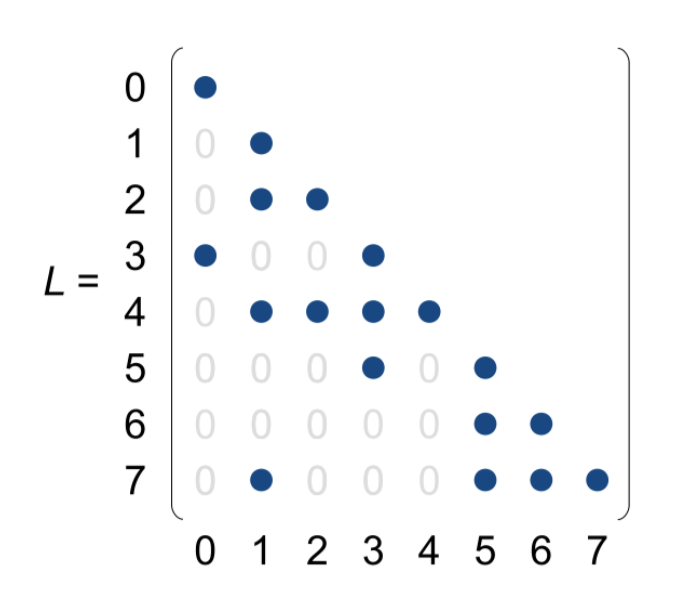
\includegraphics[height=1.3in]{Sparse_Matrix.png}
    \end{minipage}%
    }%
    \subfigure[任务依赖图]{
    \begin{minipage}[t]{0.25\linewidth}
    \centering
    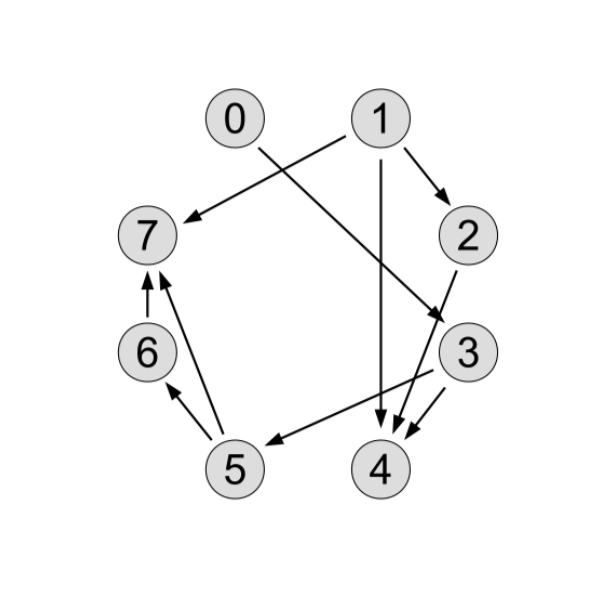
\includegraphics[height=1.3in]{DAG.png}
    \label{TDG}
    \end{minipage}%
    }%
    \subfigure[level-sets]{
    \begin{minipage}[t]{0.25\linewidth}
    \centering
    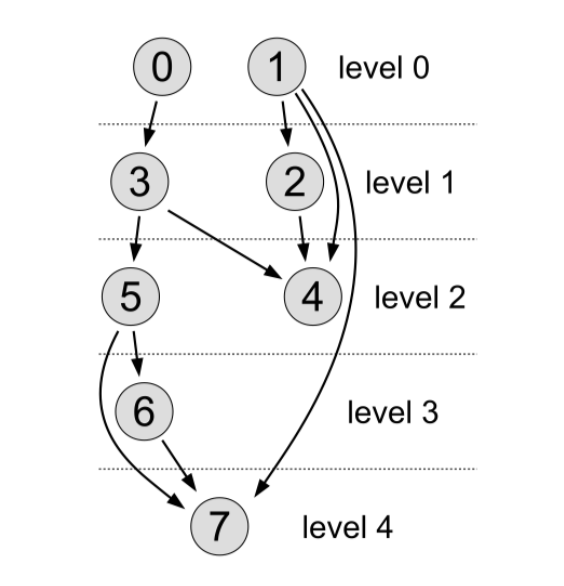
\includegraphics[height=1.3in]{level-sets.png}
    \end{minipage}
    \label{level-sets}
    }%
    \centering
\end{figure}

有研究者Saad\cite{anderson1989solving},以及Saltz\cite{saltz1990aggregation}根据SpTRSV算法是一张任务依赖图\ref{TDG}的特点,提出了基于level-sets的方法,在预处理阶段构建一个任务依赖图,如图\ref{level-sets},之后就可以在level内部进行并行,在level之间设置同步屏障,一个level执行完了再执行下一个level。

随后有研究人员基于level-sets算法,在不同的体系结构上进行了优化:CPU\cite{kabir2015sts}\cite{park2014sparsifying}\cite{Schreiber1982}\cite{wolf2010factors}以及GPU\cite{li2013gpu}\cite{naumov2011parallel}\cite{suchoski2012adapting}进行了优化。

基于level-sets的算法,存在着两个缺陷:第一,虽然可以在每个level上进行并行取得良好的并行度,但是需要在预处理阶段构建一个TAG图,计算每个任务的level,以及处理任务之间任务负载均衡的问题,在预处理阶段会花费大量的时间。写出一个有良好扩展性的并行预处理算法同样具有挑战性,往往可能会导致预处理的时间远远大于并行计算任务图的时间,在计算任务图上获得的加速甚至不能抵消预处理阶段产生的时间消耗。第二,基于level-sets的的算法需要在每个level之间都要使用一个屏障确保进行同步,等待该level内的任务都执行完了再继续下个一个任务,在负载不均衡的情况下,这会产生大量的等待时间,随着核心数量的上升,任务依赖图level数量的增加,该同步方式的时间消耗也会随之上升。

面对以上两个level-sets的缺陷,有研究人员提出了以下的优化算法。

Jongsoo Park\cite{park2014sparsifying}在基于level-sets算法进行了一些优化。他发现传统的基于level-sets的算法所使用的屏障式的同步方式会产生大量的开销。因此作者提出了一种peer-to-peer的同步方式。线程在任务执行完了之后不是等待其他线程执行到该屏障处之后再继续执行,而是会判断下一个任务的前置需求是否被完成,如果已经完成了,那么就继续运行下去。相比于基于屏障的同步方式,peer-to-peer的同步方式具有更好的扩展性。

在减少同步所需消耗方面,作者还发现,在SpTRSV算法的任务依赖图中,大部分的依赖都是多余的,作者期望通过一步预处理操作来删除这些多余依赖。例如在 2→3→5 和 2→5 这种边存在的情况下,删除了 2→5 这条边。另一方面,作者发现在这些多余依赖当中,大部分都是两跳的(比如上述的 2→5 这条边),少部分是三跳或者三跳以上。为了减少预处理的计算量,作者选择用粗略但快速的算法,只删除两跳的依赖边,而不是删除所有的多余依赖。减少了大约90\%的多余依赖,具体效果如\ref{sparsifying_edge}。该算法运行在12核的Xeon处理器上,相比于传统的基于level-sets以及屏障式同步的算法获得了至少1.6倍的加速比。

\begin{figure}[htbp]
    \centering
    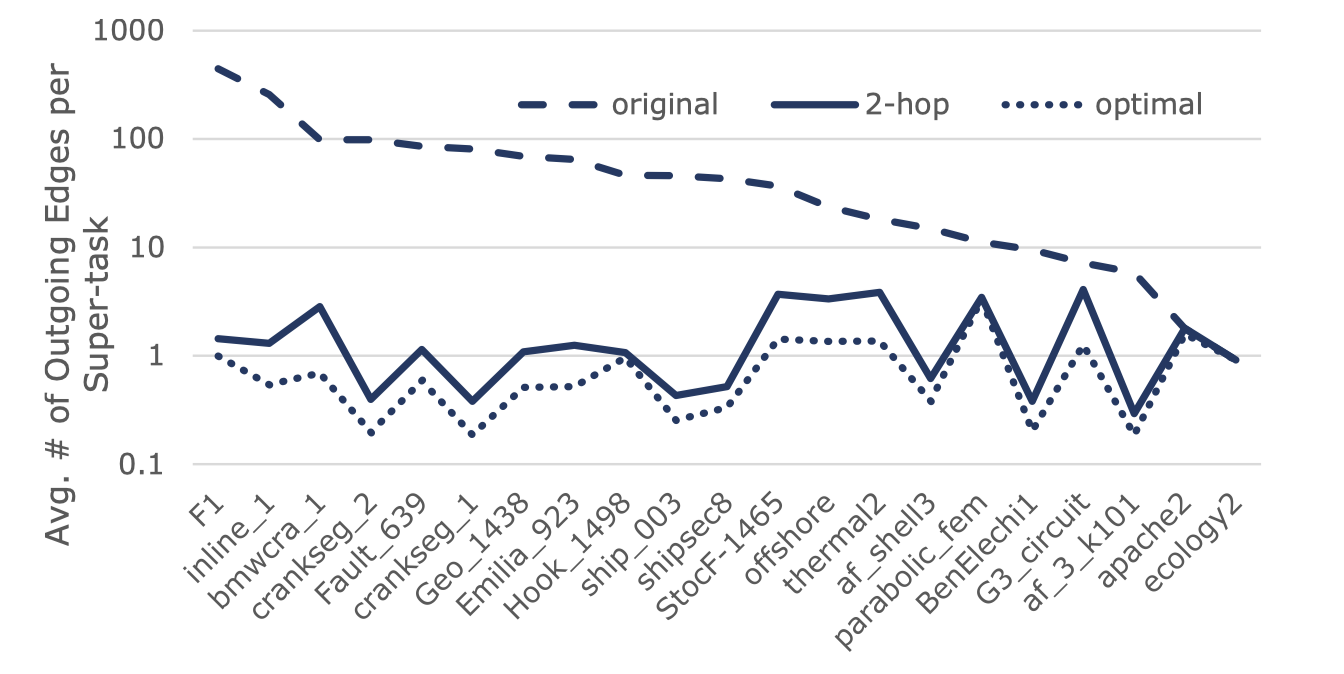
\includegraphics[width=0.7\textwidth]{sparsifying_edge.png}
    \caption{每个super-task的出度有了显著的减少}
    \label{sparsifying_edge}
\end{figure}

同时作者也做了负载均衡的优化,根据每行非零元个数的多少来进行任务的合并,组合成一定数量的super-task,使得每个super-task有相似的计算量。

刘伟峰\cite{liuSyncFree2016,liuFastSynchronizationfreeAlgorithms2017}从减少算法预处理和减少算法同步所需时间的角度出发,提出了无需同步的(synchronization-free)SpTRSV算法。 基于传统level-set的方法,随着矩阵大小的增加,其在预处理阶段所需的消耗会剧烈增加,且同步所需的时间在计算总时间中的占比也会大量增加。他的算法在 预处理阶段只计算了每个任务的 in-degree 数组(用来记录每一个节点需要有多少入度),而不是构造一个依赖图,大幅减少了预处理时间,而且该预处理方法能够轻易地使用多核来进行并行加速。对于每个 warp 使用自旋锁,不断判断前置依赖 是否都被满足来决定该结点是否开始计算。当一行计算完成后,使用原子操作来“通知”后继节点,减少了同步的时间。同时作者结合GPU的体系结构,针对GPU的片上内存和全局内存进行了优化,该算法在 GPU TitanX 上比 Nvidia 提供的算法快 2-3 倍。

\begin{figure}[htbp]
    \centering
    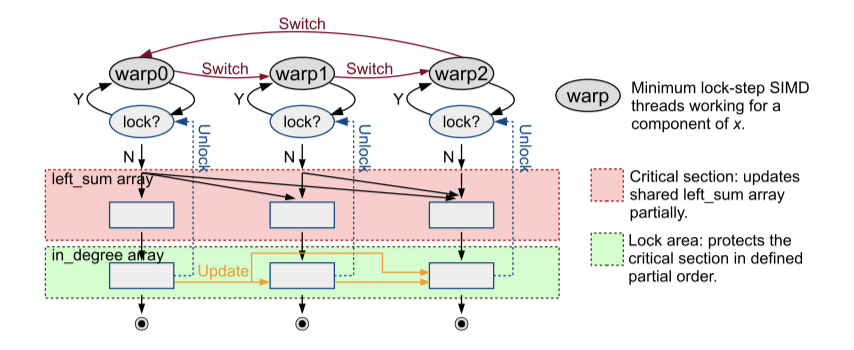
\includegraphics[width=0.7\textwidth]{sync-free.png}
    \caption{synchronization-free SpTRSV算法的示意图}
    \label{sync-free}
\end{figure}

倪鸿、刘鑫\cite{nihong2019}根据国产异构众核处理器 SW26010 体系结构的特点,针对非结构网络计算, 提出了一种基于流水线串行-局部并行思想的通用众核 SpTRSV 优化方法。首先,为了减少预处理时间,根据核心的个数,将向量 x 平均划分为多个向量块。每个向量块 x 交给一个从核进行 处理。每个从核的操作流程为:(1)等待接受来自依赖向量块的数据,直到满足进入(2)。(2)进行 x 的计算。(3)发送计算得到的 x 给需要的核心。其次,为了解决 SW26010 寄存器通讯的局限性,作者还搭建了众核通信架构。同时还有数据压缩、LDM 缓冲、访存掩盖以及数据压缩等优化。

Wang, X., Xu, P.\cite{wangFastSparseTriangular2018}等研究人员通过分析总结现有的 SpTRSV 算法,给出了一个基于生产者和消费者的统一模型,且具有一定的泛化能力。针对不同体系结构的给出了编程指导性意见。同时利用这个模型,在SW26010上提出了快速的SpTRSV算法。

\section{研究内容}

本文基于鲲鹏920处理器进行SpTRSV算法的设计与优化。研究内容包括:

\begin{enumerate} \setlength{\itemsep}{0pt}
    \item 设计一个无需预先构建任务依赖图,并且使用原子操作进行同步的SpTRSV算法。并且针对多核CPU架构的特点,以及ARMv8指令集进行优化。设计一个与华为鲲鹏平台的软硬件特性相适应的 SpTRSV 并行化方法。矩阵采用 CSC 压缩方式,将矩阵每行视作一个子任务每个任务有三种 状态:等待依赖数据,计算,结束。多个核心在任务池中并行对子任务进行如下操作:a) 自旋判断当前任务前置依赖否被满足:首先在任务入口处,自旋判断当前任务的前置依赖是否已经被满足,如果被满足则进入计算阶段。b)在计算阶段,对未知数x[i],进行求解。c) 通过原子操作,对依赖该任务对后继任务进行更新操作。
    \item 结合鲲鹏920处理器的体系结构特点以及ARMv8指令集架构进行性能优化,主要包括针对缓存的优化,针对自旋等待性能的优化,以及针对原子指令的优化。
    \item 针对NUMA架构进行优化。SpTRSV 是典型的 memory-bound 和 latency-bound 计算任务,利用 NUMA 架构可以显著提升内存带宽。目前对于 SpTRSV 算法,研究人员从任务划分、LDM 空间优化、负载均衡、自适应等角度进行了优化,取得了不错的成果。但是,缺少利用计算系统的 NUMA 特性进行优化的相关研究。本文利用操作系统提供的libnuma编程接口,根据稀疏下三角矩阵本身是只读数据的特点,将下三角矩阵分为4个副本,分配到4个NUMA结点当中。
    \item 在SpTRSV算法中在求解x[i]时,存在的向量乘法的操作,通过使用SIMD指令提升算法的性能。编译器支持自动向量化功能,其会自动利用 NEON 属性,编译时将代码向量化。启用自动向量化功能前需要打开相应的编译选项,且并非所有代码均可向量化,其需要符合一定的编码方式和规律,以提供更多的提示信息给编译器,进一步触发编译器进行代码的向量化;也可以使用 NEON intrinsic 函数进行显示的优化。NEON intrinsic 函数是一系列 C 函数 调用,编译器可将其替换为适当的 NEON 指令或 NEON 指令序列。NEON intrinsic 函数几乎提供与编写 NEON 汇编指令相同的功能,但是将寄存器分配等工作留给编译器,以便开发人 员可以专注于算法开发。与使用 NEON 汇编指令编码相比,NEON intrinsic 方式的代码有更好的可维护性。Arm 编译器、GCC 和 LLVM 编译器都支持 NEON intrinsic
    \item 通过查阅相关文献搜集测试用的矩阵,进行正确性的验证,确保算法的正确性。结合性能分析工具,分析计算的特点,对算法进行性能的调优。最后,对并行效率和算法的可扩展性进行分析。
\end{enumerate}

\section{本文组织结构}

本文基于华为鲲鹏920处理以及ARMv8架构,设计高效的并行SpTRSV算法,并结合计算系统体系结构的特点进行针对性地优化。本文的组织结构如下:

第一章绪论,主要介绍了课题背景,研究现状,研究内容,以及本文构成。在课题背景当中,本文介绍了稀疏下三角矩阵求解的研究背景、应用场景及其重要意义。在研究现状当中,分析回顾了现有国内玩研究基础、研究现状。在研究内容中,本文概括性地说明研究的重点内容,及其创新特色。

第二章介绍了相关理论与技术介绍,这里本文提到了稀疏线性方程组求解常用的方法,其中稀疏下三角矩阵的求解效率的优化对直接法和不完全乔列斯基共轭梯度下降法求解线性方程组具有重要意义。接着介绍了三种常用的稀疏矩阵压缩方式,以及本文为什么选用CSC压缩方法的原因。然后本文介绍了现存的SpTRSV算法,包括两种基于不同压缩格式的SpTRSV算法,以及在GPU和CPU上目前性能较好的SpTRSV算法。在第二章中,本文还介绍了本文所使用的优化技术及其原理,为后面算法设计打下理论基础。

第三章设计与实现了SpTRSV算法,阐述了得到下三角稀疏矩阵和进行正确性验证的方法。然后介绍了本文设计的SpTRSV算法的实现细节和优化方法。

第四章分析了算法的总体性能以及相关优化方法对性能提升的效果,以及结合理论得出的分析与思考。

第五章总结与展望,对SpTRSV算法进行了总结与分析,指出了该算法的不足之处;在未来展望部分,提出了一些可以进一步优化的优化思路。

\endinput

\chapter{相关理论与技术介绍}

\section{稀疏线性方程组求解}

经典的求解线性方程组的方法一般分为两类:直接法和迭代法。前者例如高斯消元法, LU分解等,后者的例子包括共轭梯度法等。直接法指在不考虑计算舍入误差的情况下,通过包括矩阵分解和三角方程组求解等有限步的操作求得方程组的精确解,因此又称精确法;迭代法指给定一个初始解向量,通过一定的计算构造一个向量列(一般通过逐次迭代得到一系列逼近精确值的近似解),向量列的极限为方程组理论上的精确解。

\section{稀疏矩阵的压缩方式}

存储矩阵的一般方法是采用二维数组,其优点是可以随机地访问每一个元素,因而能够容易实现矩阵的各种运算。对于稀疏矩阵,它通常具有很大的维度,有时甚大到整个矩阵(零元素)占用了绝大部分内存采用二维数组的存储方法既浪费大量的存储单元来存放零元素,又要在运算中浪费大量的时间来进行零元素的无效运算。因此必须考虑对稀疏矩阵进行压缩存储(只存储非零元素)。

\subsection{COO Format}

最简单的稀疏矩阵的存储格式称为coordinate(COO) format,这个形式只保留那些非0的值,分别使用三个数组:val, rolIdx, colIdx来对应存储数值、行号以及列号,这三个数组的大小都为矩阵非零元的个数NNZ。例如下方4x5矩阵。


$$
\begin{pmatrix}
    \label{稀疏矩阵例子}
    1 & 0 & 0 & 0 & 0 \\
    2 & 4 & 0 & 6 & 0 \\
    3 & 0 & 5 & 0 & 0 \\
    4 & 7 & 0 & 8 & 9
\end{pmatrix}
$$

~\\
~\\
~\\

该矩阵在COO存储格式下,三个数组分别为:
\begin{lstlisting}[title=COO Format]
val = {1, 2, 4, 6, 3, 5, 4, 7, 8, 9}
rolIdx = {0, 1, 1, 1, 2, 2, 3, 3, 3, 3}
colIdx = {0, 0, 1, 3, 0, 2, 0, 1, 3, 4}
\end{lstlisting}

\subsection{CSR Format}

CSR(Compressed Sparse Row)是一种按行压缩的矩阵存储形式。分别使用三个数组:val, rowPtr, colIdx来对应存储数值、行指针、以及列号。其中val和colIdx的数组大小为非零元的个数NNZ,而rowPtr数组的大小一般为m+1,其中 m 为矩阵行的个数。例如图\ref{CSR}。

\begin{figure}[htbp]
    \centering
    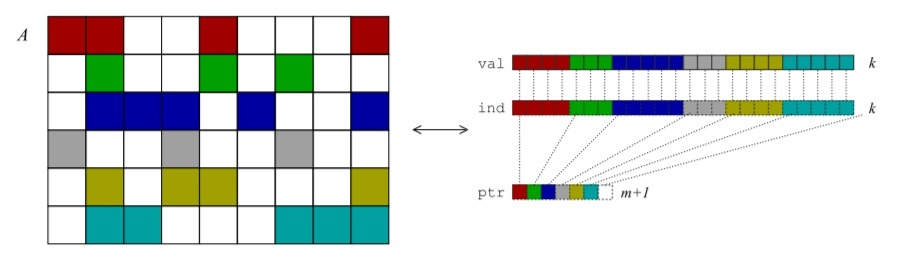
\includegraphics[width=0.7\textwidth]{CSR.png}
    \caption{CSR矩阵存储格式}
    \label{CSR}
\end{figure}

\subsection{CSC Format}

CSC(Compressed Sparse Column)与CSR相似,是一种按列压缩的矩阵存储格式。分别使用是那个数组:val, colPtr, rowIdx来对应存储数值、列指针、以及行号。其中val和rowIdx的数组大小为非零元的个数NNZ,而colPtr数组的大小一般为n+1,其中n为矩阵列的个数。例如图\ref{CSC}

\begin{figure}[htbp]
    \centering
    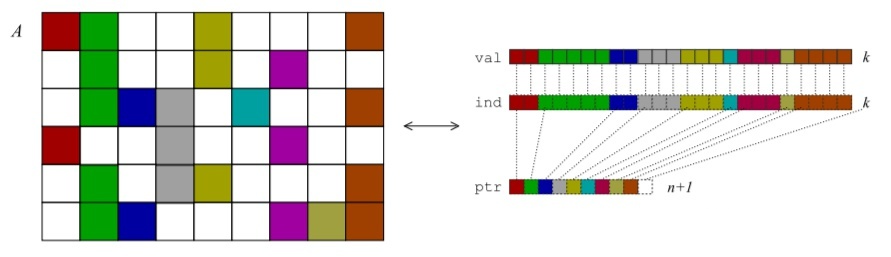
\includegraphics[width=0.7\textwidth]{CSC.png}
    \caption{CSC矩阵存储格式}
    \label{CSC}
\end{figure}

\section{已有SpTRSV算法}

\subsection{基于CSR格式的SpTRSV串行算法}

\begin{algorithm}[H]
    \caption{CSR Based Serial SpTRSV}\label{csr-serial-sptrsv}
    MALLOC(*left\_sum, n) \;
    MEMSET(*left\_sum, 0) \;
    \For{i = 0; i < n; i++}{
        \For{j = row\_ptr[i] ; j < row\_ptr[i + 1] - 1 ; j++}{
            left\_sum[i] \small{$\leftarrow$} left\_sum[i] + val[j] \small{$*$} x[col\_idx[j]] \;
         }
        x[i] \small{$\leftarrow$} (b[i] - left\_sum[i]) / val[col\_ptr[i]] \;
    }
\end{algorithm}

基于CSR格式的SpTRSV串行算法第一个循环从矩阵的第0行开始遍历这个矩阵。在第二个循环进行向量乘法的操作,求出left\_sum[i]。之后再求出未知数x[i]。

\subsection{基于CSC格式的SpTRSV串行算法}

\begin{algorithm}
    \caption{CSC Based Serial SpTRSV}\label{csc-serial-sptrsv}
    MALLOC(*left\_sum, n) \;
    MEMSET(*left\_sum, 0) \;
    \For{i = 0; i < n; i++}{
        x[i] \small{$\leftarrow$} (b[i] - left\_sum[i]) / val[col\_ptr[i]] \;
        \For{j = col\_ptr[i] + 1 ; j < col\_ptr[i + 1] ; j++}{
            left\_sum[rowIdx[j]] \small{$\leftarrow$} left\_sum[row\_idx[j]] + val[j] \small{$*$} x[i] \;
        }
    }
\end{algorithm}

该算法的第一个循环从矩阵的第0行开始遍历这个矩阵。首先求出该算该行未知数$x[i]$,接着遍历该列的上的非零元,对该列非零元所对应的$left\_sum$进行更新,$left\_sum[rowIdx[j]] += val[j] \times x[i]$。

基于CSR压缩格式SpTRSV算法以及基于CSC压缩格式的SpTRSV算法,两者在访存模式上存在着一定的差异。基于CSR格式的算法需要进行频繁离散读取未知数向量x[col\_idx[j]],相反基于CSC格式的SpTRSV算法只需要读取当前行号 i 所对应的x[i]。在写数据方面,基于CSR的并行算法需要集中的写left\_sum[i]的数据,而基于CSC的并行算法则是离散的写left\_sum[rowIdx[j]],在多核运算的条件下,离散的写比集中的写同一位置的数据更容易进行并行化。

\subsection{基于level-sets的SpTRSV并行算法}

J.Park在level-sets算法的基础上提出除了更高效的并行SpTRSV算法\cite{park2014sparsifying},该算法主要分为两个阶段:预处理阶段和计算阶段。

在预处理阶段主要有三个处理步骤:
\begin{enumerate} \setlength{\itemsep}{0pt}
\item 使用由Chhugani\cite{chhuganiFastEfficientGraph2012a}提出的高度优化的并行广度优先搜索算法(BFS),构建了一个任务依赖图\ref{TDG}。
\item 在任务依赖图的基础上,作者又通过将同level的任务合并为super-task的形式实现负载均衡,确保每个线程被分配有相似计算量的super-task,这种合并的操作有进一步减少了任务之间的依赖个数,进一步减少了同步所需的消耗。
\item 作者发现任务依赖图中存在着大量的多余依赖边,并开发了一个高效的过滤算法,去除了两条的依赖边。
\end{enumerate}

在计算阶段作者使用了与传统level-sets算法不同的调度方式,作者使用peer-to-peer的同步方式替换为了在level之间使用屏障\ref{Level-scheduling with barrier}进行同步的方式。下面是两种不同同步方式的伪代码:算法\ref{Level-scheduling with barrier}、算法\ref{Level-scheduling with peer-to-peer synchronization}

\begin{algorithm}
    \caption{Level-scheduling with barrier}
    \label{Level-scheduling with barrier}
    \ForEach{level l}{
        solve the unknowns of \small{$task_{l}^{t}$} \;
        barrier;
    }
\end{algorithm}
\begin{algorithm}
    \caption{Level-scheduling with peer-to-peer synchronization}
    \label{Level-scheduling with peer-to-peer synchronization}
    \ForEach{level l}{
        wait until all the parents are done wait \;
        solve the unknowns of \small{$task_{l}^{t}$} \;
        \textbf{done}[\small{$task_{l}^{t}$}] \;
    }
\end{algorithm}

对比两种不同的调度算法,可以发现使用peer-to-peer的调度方式,能够使得计算资源能够得到更好的利用。因为当一个线程完成任务计算之后,基于屏障的同步方式会让该线程进入等待的状态。而基于peer-to-peer的调度方式则会让该线程继续进行下去。如图\ref{两种不同同步方式的对比示意图},如果采用基于peer-to-peer的同步方式,线程2在完成任务2之后可以不用等在线程1完成任务1,可以接着运行下去。这在一定程度上也有利于负载均衡。

\begin{figure}[htbp]
    \centering
    \subfigure[通过屏障同步]{
    \begin{minipage}[t]{0.30\linewidth}
    \centering
    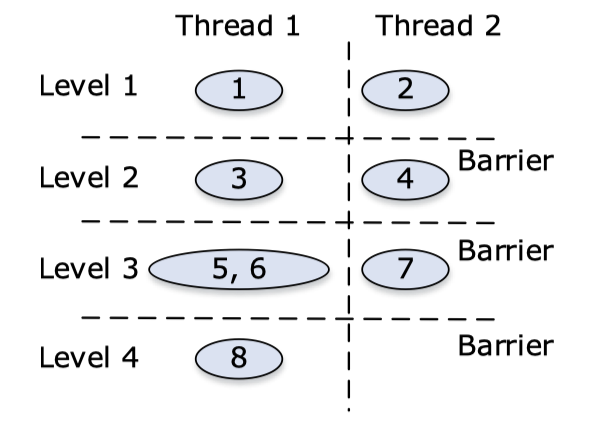
\includegraphics[height=1.3in]{sync-barrier.png}
    \end{minipage}%
    }%
    \subfigure[点对点同步]{
    \begin{minipage}[t]{0.30\linewidth}
    \centering
    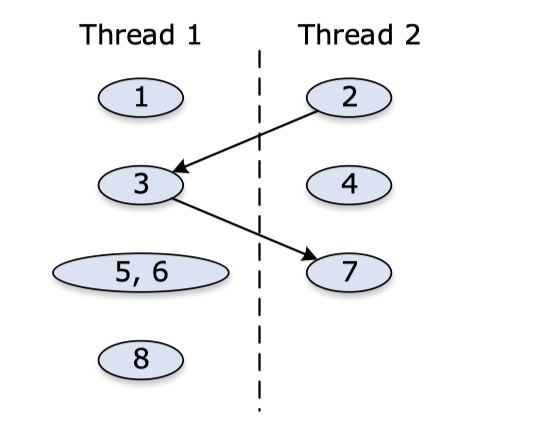
\includegraphics[height=1.3in]{sync-p2p.png}
    \label{TDG}
    \end{minipage}%
    }%
    \centering
    \caption{两种不同同步方式的对比示意图}
    \label{两种不同同步方式的对比示意图}
\end{figure}

\subsection{sync-free的SpTRSV并行算法}

\begin{table}[]
    \caption{基于level-sets算法\cite{park2014sparsifying}的任务耗时(ms)分解表}
    \label{任务耗时分解图}
    \resizebox{\textwidth}{!}{%
    \begin{tabular}{|l|l|l|l|l|l|}
    \hline
    \multirow{2}{*}{矩阵名称} &
      \multirow{2}{*}{预处理时间} &
      \multirow{2}{*}{SpTRSV计算阶段花费时间} &
      \multicolumn{2}{l|}{SpTRSV计算阶段时间分解} &
      \multirow{2}{*}{level的个数} \\ \cline{4-5}
     &
       &
       &
      同步时间消耗 &
      计算时间消耗 &
       \\ \hline
    \begin{tabular}[c]{@{}l@{}}FEM/ship 003 \\ FEM/Cantilever \\ chipcool0 \\ nlpkkt160\end{tabular} &
      \begin{tabular}[c]{@{}l@{}}92.46\\ 47.89\\ 8.74\\ 484.67\end{tabular} &
      \begin{tabular}[c]{@{}l@{}}12.95\\ 9.60\\ 1.99\\ 38.30\end{tabular} &
      \begin{tabular}[c]{@{}l@{}}10.96\\ 5.62\\ 1.15\\ 0.01\end{tabular} &
      \begin{tabular}[c]{@{}l@{}}1.99\\ 3.98\\ 0.84\\ 38.29\end{tabular} &
      \begin{tabular}[c]{@{}l@{}}4367\\ 2397\\ 534\\ 2\end{tabular} \\ \hline
    \end{tabular}%
    }
\end{table}


基于level-sets的算法需要花费大量的时间在预处理和任务间的同步上,运行J.Park的算法并分步进行统计(预处理阶段,同步所需耗时,计算阶段),我们就可以得到表\ref{任务耗时分解图}。所用的稀疏矩阵来自于佛罗里达大学的稀疏矩阵集合\cite{davis2011university},观察这张表我们可以主要得到以下几点信息:
\begin{enumerate} \setlength{\itemsep}{0pt}
\item 预处理阶段所消耗的时间,要远大于计算阶段所消耗的时间,平均大概是8至10倍左右。预处理占总时间大约80\%。
\item 同步所需的开销会导致的时间消耗,会随着矩阵level个数的增加而剧烈增加,当稀疏矩阵的level较多时,会导致同步的时间消耗远大于计算的时间消耗。这也可能是同level间负载不均衡所导致的。
\end{enumerate}

例如nlpkkt160只有两个level,同步所占用的时间要远小于计算所需的时间。作为对比矩阵FEM/ship 003,虽然矩阵的规模小于lpkkt160,但是由于其level相对较多,导致了同步所占用的时间也较多。

刘伟锋从减少预处理和减少同步所需时间的角度出发,提出了名为sync-free的SpTRSV计算方法\cite{liuSyncFree2016}。该算法能够在GPU上能够取得较好的效果。与传统基于level-sets的算法不同的是,sync-free的SpTRSV算法只在预处理阶段计算每个任务的入度,该入度表示当前任务有多少的前置依赖。作者使用一个warp,32个线程来处理每个任务。任务之间通过使用共享变量以及原子操作的方式,来决定任务之间的顺序。算法的伪代码见\ref{sync-free alogrithm preprocess}ref{sync-free alogrithm solve}

\begin{algorithm}[htbp]
    \caption{sync-free SpTRSV预处理阶段算法}
    \label{sync-free alogrithm preprocess}
    \SetKw{atomic-add}{atomic-add} 
    \SetKw{atomic-sub}{atomic-sub} 
    \SetKw{Parallel}{Parallel} 
    \SetKwProg{Fn}{Function}{ is}{end}
    malloc(*d\_left\_sum, *s\_left\_sum, *d\_in\_degree, *s\_in\_degree, n)\;
    memset(*d\_left\_sum, *s\_left\_sum, *d\_in\_degree, *s\_in\_degree, 0)\;
    \Fn{Preprocess()}{
        \Parallel \For{i = 0; i < nnz; i++}{ 
            atomic-add(\&d\_in\_degree[row\_idx[i]], 1) \; 
        }
    }
\end{algorithm}

\begin{algorithm}[htbp]
    \caption{sync-free SpTRSV计算阶段的算法}
    \label{sync-free alogrithm solve}
    \SetKw{atomic-add}{atomic-add} 
    \SetKw{atomic-sub}{atomic-sub} 
    \SetKw{Parallel}{Parallel} 
    \SetKwProg{Fn}{Function}{ is}{end}

    \Fn{Solve()}{
        \Parallel \For(using one warp for one entry){int i = 0; i < n; i++}{
            \While(test dependencies){s\_in\_degree[i] + 1 \small$\neq$ d\_in\_degree[i]}{
                // busy wait \;
            }
            \small{$x[i] \leftarrow (b[i]-d\_left\_sum[i] - s\_left\_sum[i])/val[col ptr[i]]$}\;
            \Parallel \For(one thread for one nonzero){j in \small{$[col\_ptr[i]+1], col\_ptr[i+1]-1$}}{
                \uIf{in local}{
                    atomic-add(\&s\_left\_sum[rid], \small{$val[j] \times x[i]$}) \;
                    atomic-add(\&s\_in\_degree[rid], 1) \;
                }
                \Else{
                    atomic-add(\&s\_left\_sum[rid], \small{$val[j] \times x[i]$}) \;
                    atomic-add(\&s\_in\_degree[rid], 1) \;
                }
            }

        }

    }
    
\end{algorithm}

\section{基于缓存的优化技术}

\subsection{内存cache}

\begin{figure}[htbp]
    \centering
    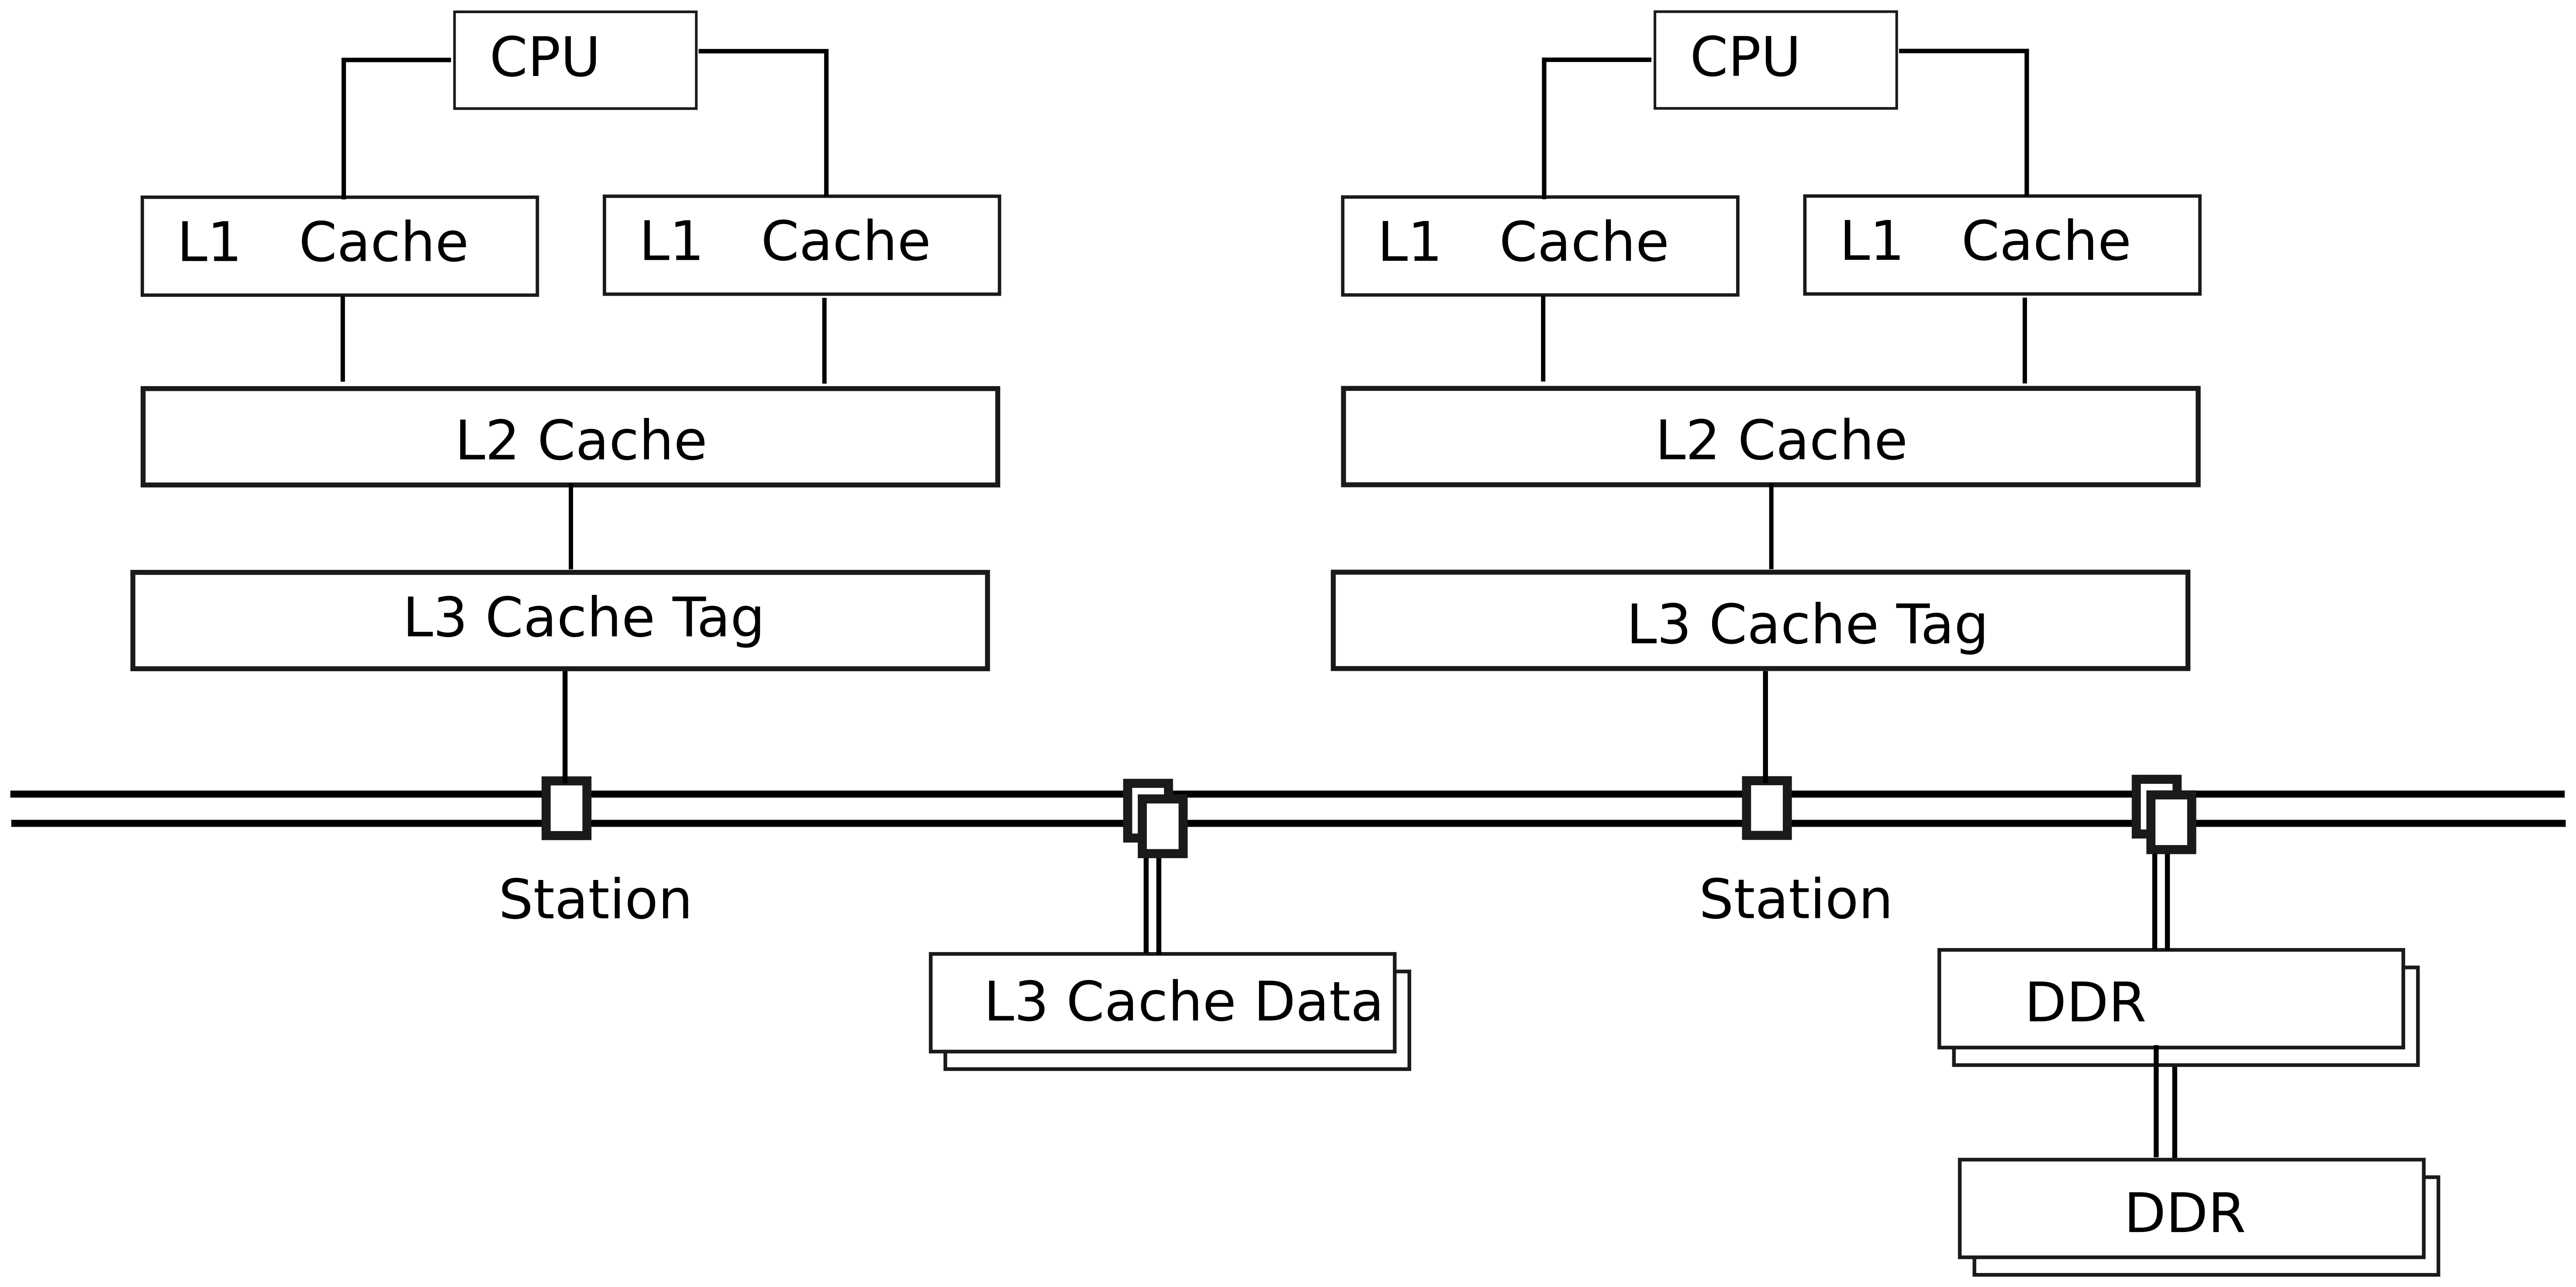
\includegraphics[width=0.7\textwidth]{kp920_cache.png}
    \caption{kunpeng cache示意图}
    \label{Kunpeng Cache示意图}
\end{figure}


Cache在计算机系统中,是一种基于分层优化思想的一种优化手段。由于CPU的速度远大于内存的速度,出于成本的考虑,人们常用相对高速的Cache来弥补两者之间的差距,提升CPU的性能。

图\ref{Kunpeng Cache示意图}为鲲鹏920处理器内存Cache的示意图\cite{kunpeng920pub},在鲲鹏920芯片中,每个核心独占L1、L2两级缓存。离核心最近的是两个L1 Cache,分开缓存指令和数据,大小分别为64K。L2 Cache则要大得多,大小为512k。而第三级缓存则是鲲鹏920芯片上的所有核心共享,其中L3 Cacheline的长度为128个字节。

\subsection{Cache Prefetch}
Cache Prefetch也是一个针对Cache的优化设计。Cache比实际的内存快很多,所以如果我们可以提前加载部分内存到Cache中,就会在性能上有优势。比如一个乘法的时间,就算不考虑流水线,也不过3-12个周期,但是从DDR内存中读取数据可能会花费100个始终周期。所以最好还是在计算开始前,先让数据从内存加载到缓存当中,做到计算和缓存同步进行。

例如,如下代码:
\begin{lstlisting}[language=c++]
    for (i=0; i<W; i++) {
        for(j=0; j<W; j++) {
          c[i][j] = 0;
          if (!(j%INT_PER_CACHELINE))
                  __builtin_prefetch((const void *)&c[i][j+INT_PER_CACHELINE], 1, 3);
          for (k=0; k<H; k++) {
                  c[i][j] += a[i][k]*b[k][j];
                  if (!j && !(k%INT_PER_CACHELINE))
                          __builtin_prefetch((const void *)&a[i][k+INT_PER_CACHELINE], 0, 3);
                  if (!i && !(j%INT_PER_CACHELINE))
                          __builtin_prefetch((const void *)&b[k][j+INT_PER_CACHELINE], 0, 3);
          }
        }
  }
\end{lstlisting}

这里的\_\_builtin\_prefetch是gcc的内置函数,在不同的平台有不同的封装。在上面的算法中,我们进行某个向量单元的计算的时候,已经可以知道后面要计 算的内存单元是什么了,我们就可以提前把数据取出来。除了软件在做prefetch外,鲲鹏920处理器中也有硬件实现的prefetch单元,如\ref{hw_prefetch}。这就导致软件层面的prefetch可以没有很好的效果。

\begin{figure}[htbp]
    \centering
    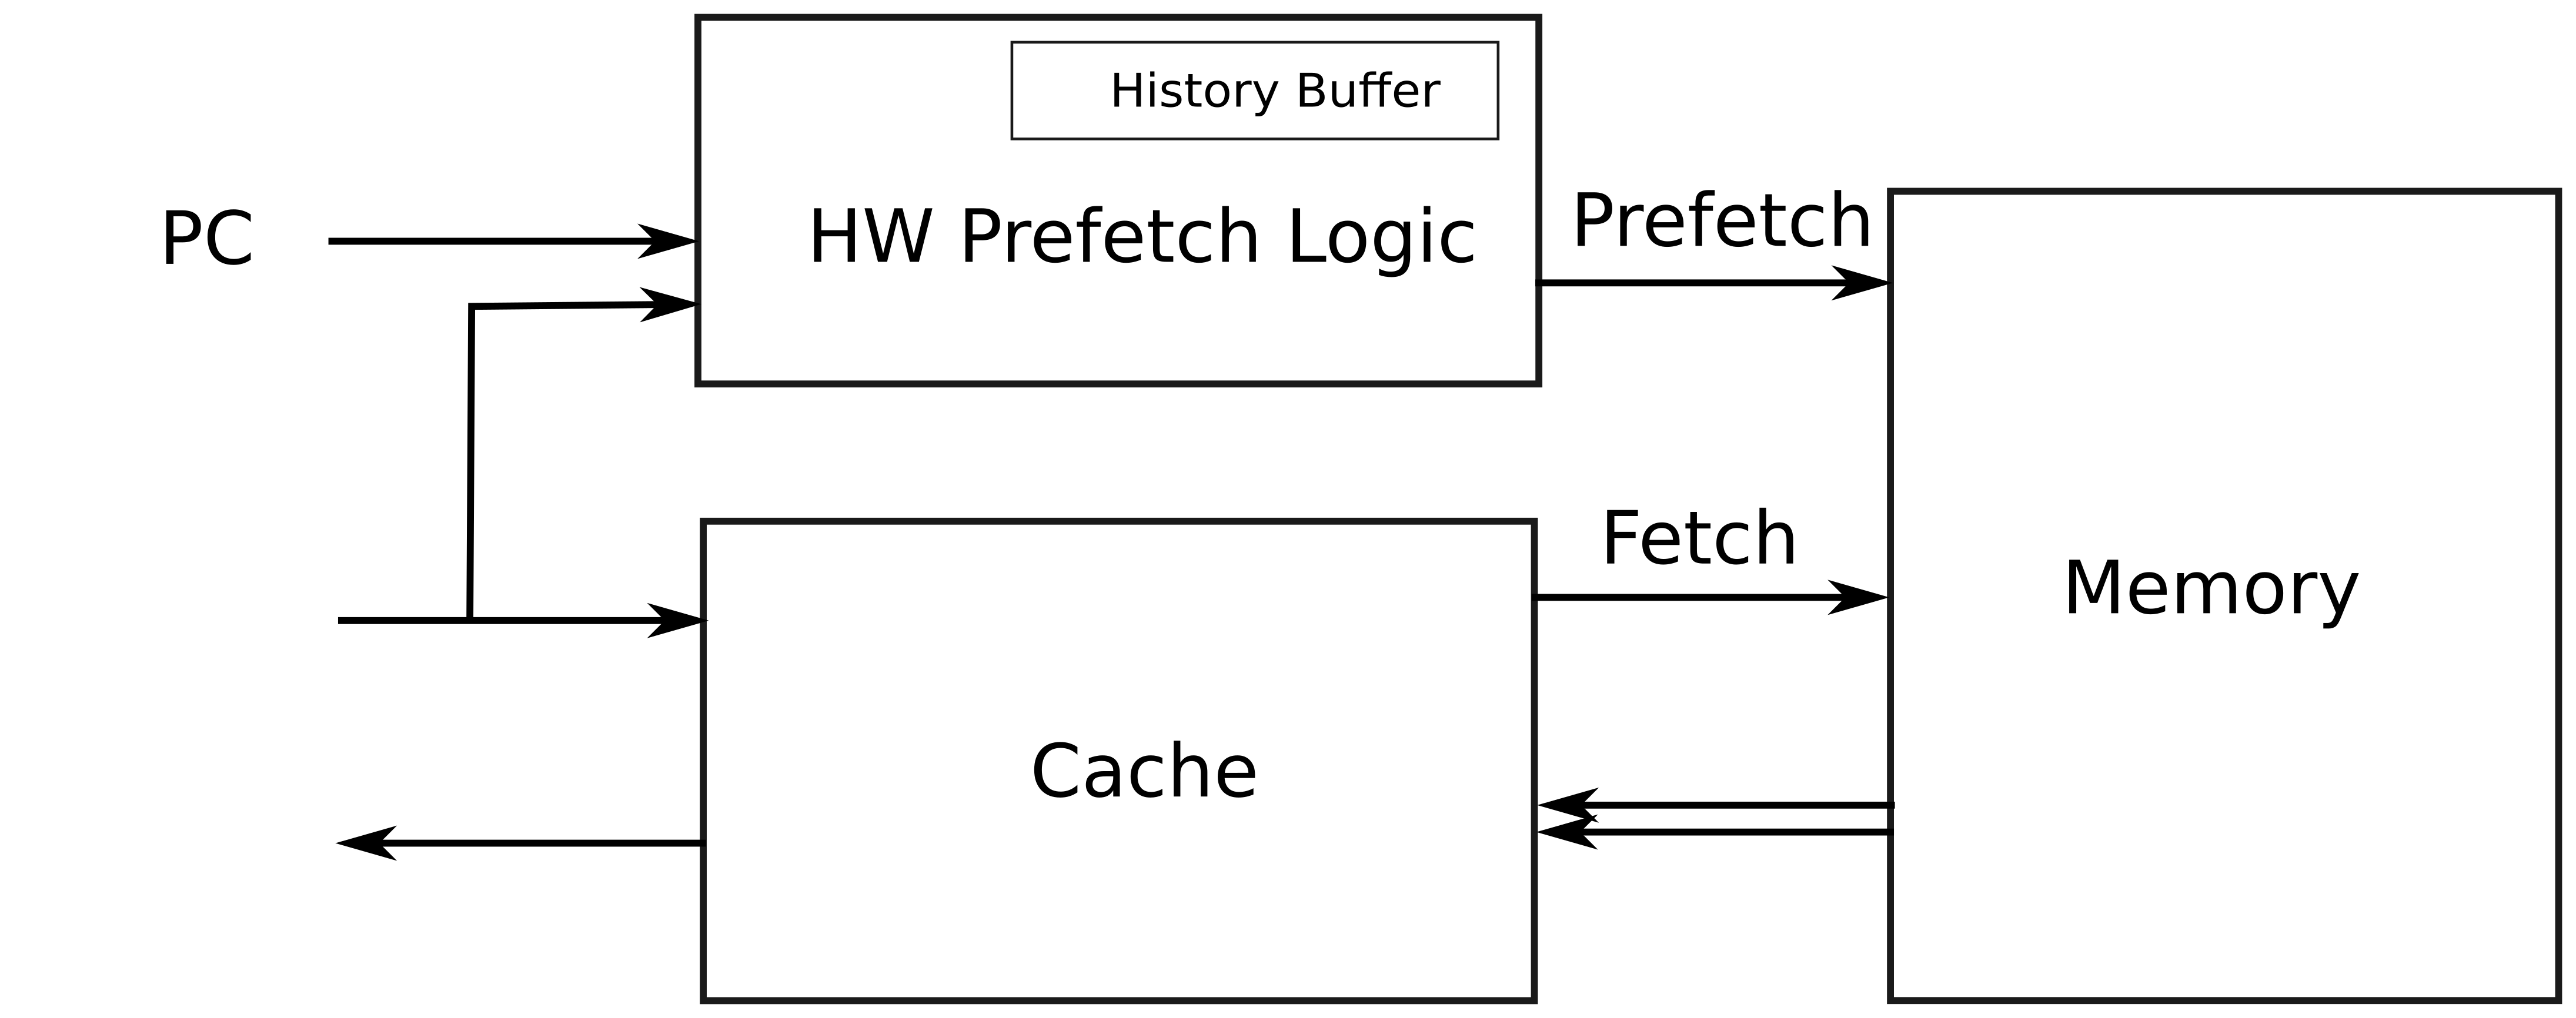
\includegraphics[width=0.7\textwidth]{hw_prefetch.png}
    \caption{鲲鹏920 cache prefetch的硬件结构示意图\cite{kunpeng920pub}}
    \label{hw_prefetch}
\end{figure}

\subsection{缓存一致性协议}

在多核CPU的情况下,由于每个核心都有自己的独占的缓存,数据在这些缓存中制造了多个备份,这就造成了,到底哪份有效的问题。鲲鹏920采用的是监听一致性协议(Snooping),该协议是通过总线广播的形式实现的。最为经典的监听一致性协议是MESI,该协议由 James Goodman 提出,目前已在x86、ARM、Power架构中得到实现。

MESI协议将CacheLine分为四个状态
\begin{enumerate} \setlength{\itemsep}{0pt}
\item Modified(M):该状态表示,此CacheLine有效,数据只存在本cache中,且CacheLine中的数据被修改和内存中的不一样。在这种状态下,如果监听到有其他芯片读取缓存行对应主存的操作,该操作就会被延迟:首先将该操作写回,然后本CacheLine的状态就会变为S。
\item exclusive(E):该状态表示,此CacheLine有效,数据只存在于本cache中,数据和Cache中的数据和对应内存中的数据一致。如果监听到总线中其他线程对该行的读取操作,状态将变为S。
\item Shared(E):该状态表示,此CacheLine有效,数据存在于多个Cache中。如果监听到有其他线程的修改或独享请求,那么改缓存行就变为无效
\item Invalid(I):该状态表示,此CacheLine无效,如果有线程对该数据进行读取,就触发cache miss,重新从内存中读取对应的数据。

\end{enumerate}
此外还有一种基于目录是的MESIF缓存一致性协议,这里就不详细展开,详见\cite{husengseng2017}。

总线本质上是一个去中心化的系统,随着核心数量的增加,维护缓存一致性的成本也会增加。例如,假设32个线程同时在一个变量上做自旋锁的操作,此时如果有一个核心更新了一次spinlock,那么就要通知另外31个线程。如果总线上发生了冲突,会导致计算性能进一步下降。

\subsection{伪共享}
缓存一致性协议以及数据按照CacheLine大小读取到Cache,这两个特点造成了在多核计算中经常出现的问题:伪共享(false sharing)。

\begin{lstlisting}[language=c++]
    #omp parallel for num_threads(10)
    for(int i = 0; i < 10; i++){
        for(int j = 0; j < 10; i++){
            sum[i] += i * j;
        }
    }
\end{lstlisting}

例如上述代码,在鲲鹏920中,CacheLine的大小为128字节,sum数组可能会被分配掉同一个CacheLine中,这种情况下,会导致算法的并行度无法上升。因为一个核心的写操作都会导致其他核心的缓存失效。当其他线程需要读写该区域内存的时候需要首先将修改过的CacheLine写回,然后重新从内存中读取。

通常可以通过padding的方式来解决伪共享的问题,如图\ref{通过padding的方式解决伪共享导致的问题}。对于多线程频繁读写的数据,通过padding,将不想管的数据分配到不同的CacheLine当中。

\begin{figure}[htbp]
    \centering
    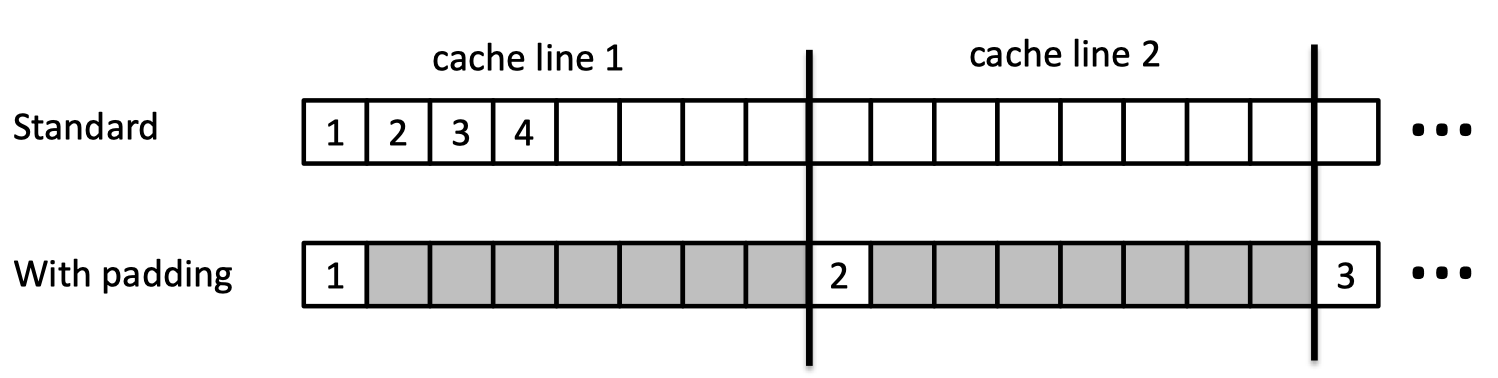
\includegraphics[width=0.7\textwidth]{CacheLine.png}
    \caption{通过padding的方式解决伪共享导致的问题}
    \label{通过padding的方式解决伪共享导致的问题}
\end{figure}

\section{ARM Neon指令}

鲲鹏920处理器基于ARMv8,支持128bits的SIMD指令。它通过在64bits的D寄存器和128bits的Q寄存器上进行向量化的操作,来实现单指令多数据运算。鲲鹏920处理器一共有16个Q寄存器和32个D寄存器。图\ref{SIMD}显示了指令$VADD.I16 Q0, Q1, Q2$同时进行了8路16bit整数的加法操作,相比于传统的加法指令有显著的性能提升。
\begin{figure}[htbp]
    \centering
    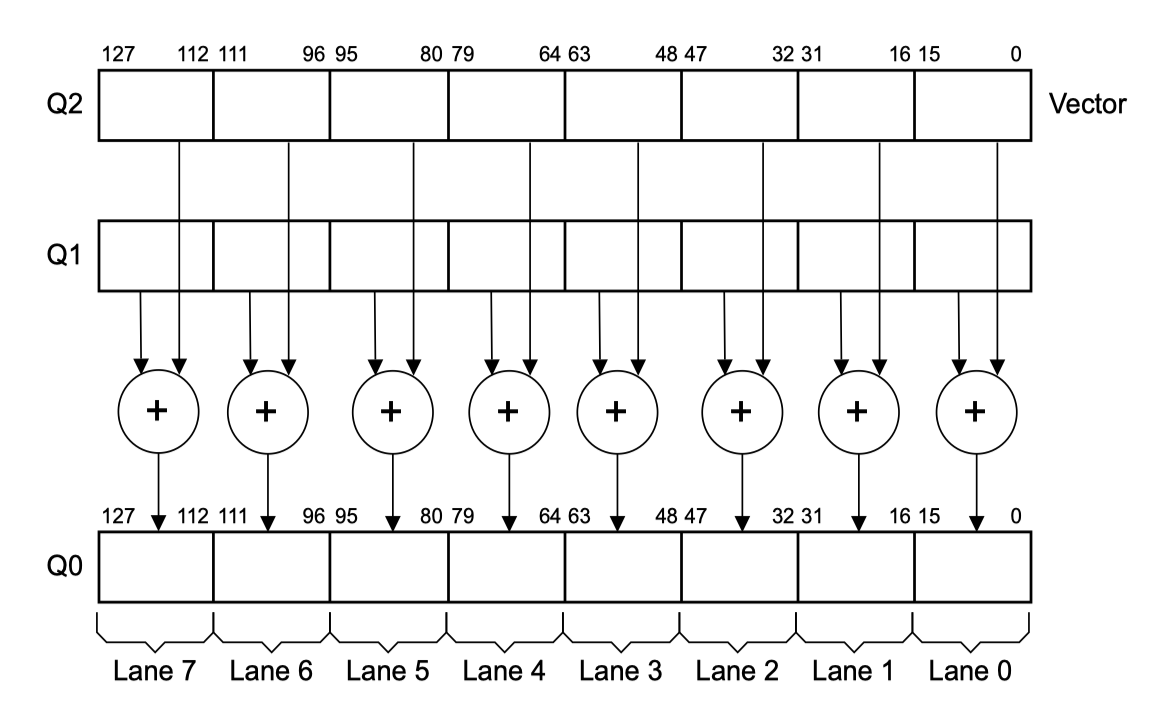
\includegraphics[width=0.7\textwidth]{SIMD.png}
    \caption{8路16位加法操作}
    \label{SIMD}
\end{figure}
ARM Neon除了提供汇编指令之外,还提供了C风格的编程接口Neon intrinsics。相比与Neon汇编指令,使用Neon intrinsics可以不用考虑寄存器的分配问题,这部分由编译器来实现,用户只需要关注上层代码。同时,也能享受编译器带来的一些优化。Neon intrinsics了丰富的编程接口,包括:对数据进行的load与store,各种常用的运算,变量常量的创建等。Neon intrinsics支持GCC编译器,使用时只需include头文件arm\_neon.h。

\section{NUMA架构}

传统多核处理器通常采用SMP(Symmetric Multi-Processing,对称多处理器)\ref{SMP架构示意图},在该架构下,每个线程的地位都是均等的,对内存使用的延迟与带宽也相同。在操作系统的支持下能够做到很好的负载均衡。鲲鹏处理器支持NUMA(Non-uniform memory access, 非统一内存访问)架构,如图\ref{NUMA架构示意图}。使用这种架构能够解决处理器核数限制的问题,同时,通过合理的软件设计,能够提升内存的带宽,解决SMP架构下总线瓶颈的问题。
\begin{figure}[htbp]
    \centering
    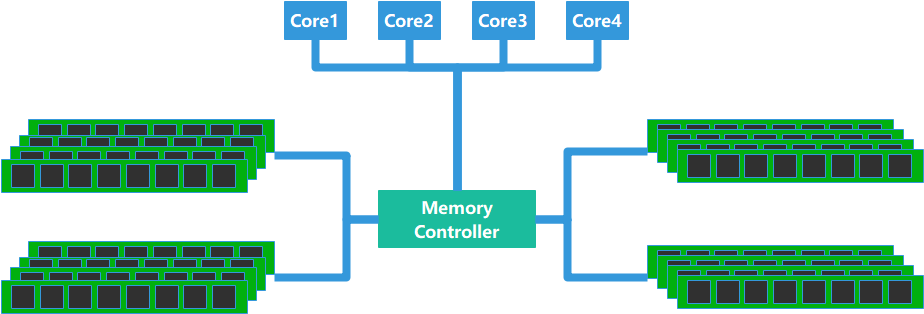
\includegraphics[width=0.7\textwidth]{SMP.png}
    \caption{SMP架构示意图}
    \label{SMP架构示意图}
\end{figure}

由于在NUMA架构下,多个核心组成一个节点(Node),系统中可以存在着多个节点,每个节点上有一个内存控制器,管理控制一片内存。内存在物理上是分布式的,通过片间网络互联。这就导致了,每个线程访问内存的延迟与带宽取决于软件相对于内存的位置,对软件设计者提出了挑战。

\begin{figure}[htbp]
    \centering
    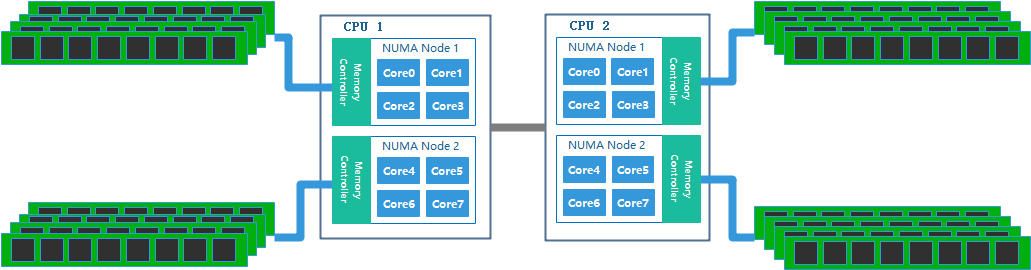
\includegraphics[width=0.7\textwidth]{NUMA.png}
    \caption{NUMA架构示意图}
    \label{NUMA架构示意图}
\end{figure}

linux从内核版本2.5开始就支持NUMA架构\cite{numalinux},用户可以通过numactl命令来手动分配程序的NUMA访问策略,例如我们可以将进程或者内存固定在指定的节点上。系统默认的NUMA策略是nodelocal,及总是在线程执行的地方分配内存。用户可以设置为numactl --interleave,这时操作系统将会在各个节点之间,使用round-robin算法均衡分配内存。同时系统也为用户提供了libnuma这一编程接口\cite{libnuma},方便用户在程序语言层面,对数据进行操作,例如手动指定数据所在的节点。

值得一提的是,默认NUMA策略下,操作系统使用的是“Fist touch”的NUMA分配原则,即用户使用malloc时操作系统会分配逻辑内存页,当初次访问这个数据时(例如初始化操作),操作系统发现该逻辑页面还没有被分配物理页面,于是就进行分配物理页面的操作,此时操作系统的根据调用线程的NUMA分配策略来进行物理页面的分配。这时,在默认NUMA分配政策下,操作系统会将数据分配到,离该线程最接近的NUMA节点。当然也可以开启numactl --interleave,来替换覆盖“First touch”的原则。

常用的编程工具OpenMP也提供了NUMA编程的接口。主要是通过两个环境变量,OMP\_PLACES决定了线程能够创建的位置,可以指定具体的节点,也可指定具体的核心。OMP\_PROC\_BIND可以设置线程的分配方式。

\section{ARMv8原子指令优化}

原子操作是多核程序中一个很重要的操作。x86通常使用锁总线的方式实现原子指令,保证了原子指令的执行期间不会收到其他指令的干扰。

在ARMv8.1发布之前,ARM处理器实现原子操作的方式是ll/sc(Load-Link/Store-Conditional),具体指令就是LDREX/STREX。

具体原理为,当CPU-A调用LOADEX命令的时候,会将数据从内存中读取到缓存当中,并将该缓存的状态标记为EX(Exclusive),此时如果还有一个CPU-B也使用了LOADEX命令,读取同一个数据,这时CPU-B中的标记变成了EX,而CPU-A中缓存行的标记则变成了S。在CPU-A执行完了之后如果要调用STREX指令,将数据写回内存,它首先检查标记的情况,发现自己没了EX,于是写回失败。重新执行LOADEX,操作数据,STREX这样的循环。而CPU-B则可以成功进行STREX,然后放弃EX标记。CPU-A不断处于循环状态,这样就会导致性能的损失。

随着ARM处理器核心数量的提升,原先LL/SC方式的原子操作通过争抢的方式获得原子操作会对性能造成很大的影响。因此,为了支持这种大型系统,在其ARMv8.1规范中引入了LSE (Large System Extensions),加入了大量原生原子操作指令\cite{ArmArchitectureReference},大致原理就是将原子操作放到存储端去做,从而提升多核计算性能,理论上在多核系统的条件下,LSE指令的性能要好与ll/sc原子指令。新的扩展指令包含CAS, SWP和LD/ST<OP>等,其中<op>为ADD,CLR,SET等。

gcc也充分利用了这一特性,提供了基于LSE原子指令的优化。

\begin{lstlisting}[caption={基于LL/SC的原子指令}]
    __LL_SC_PREFIX(arch_atomic_##op(int i, atomic_t *v))			
    {									
        unsigned long tmp;						
        int result;                               
        asm volatile("// atomic_" #op "\n"				
    "	prfm	pstl1strm, %2\n"    
    "1:	ldxr	%w0, %2\n"    
    "	" #asm_op "	%w0, %w0, %w3\n"     				
    "	stxr	%w1, %w0, %2\n"     
    "	cbnz	%w1, 1b"	   
        "=&r" (result), "=&r" (tmp), "+Q" (v->counter)	
        : "Ir" (i));
    }
\end{lstlisting}

\begin{lstlisting}[caption={基于LSE的原子指令}]
    static inline void arch_atomic_##op(int i, atomic_t *v)			
    {									
        register int w0 asm ("w0") = i;					
        register atomic_t *x1 asm ("x1") = v;				
                                        
        asm volatile(ARM64_LSE_ATOMIC_INSN(__LL_SC_ATOMIC(op),		
    "	" #asm_op "	%w[i], %[v]\n")					
        : [i] "+r" (w0), [v] "+Q" (v->counter) 				
        : "r" (x1)   					
        : "x16", "x17", "x30");  					
    }
\end{lstlisting}

对比上述两个不同的实现方式,原来基于LL/SC实现的原子操作,需要先LDXR,然后执行STXR并查看是否成功,如果不成功那就重新循环执行,直到成功。而基于LSE原子指令的实现则更加简洁,如果是atomic\_add操作只需一条LDADD指令。

\section{CPU松弛技术}

在自旋等待中,常常会使用到CPU\_relax()进行优化。也就是在自旋的循环体重插入nop操作,让cpu进行空转。在核并行的情况下,这种操作能够减轻为了维护内存序带来的性能损失。intel处理器从Pentium4开始引入了PAUSE汇编指令。在ARM架构下也能通过汇编实现类似的操作。memory指令是内存屏障的操作,保持CPU空转,在运行时防止对内存的操作乱序执行,并且会将所有缓存在寄存器中的所有变量写回内存当中,然后重新从内存中读取。


\begin{lstlisting}[language=c++]
    inline void PauseCPU() { 
        __asm__ __volatile__("yield" : : : "memory"); 
    }
\end{lstlisting}

\section{本章小结}

本章介绍了SpTRSV算法的应用场景,在线性方程求解算法中,LU分解和预优化的共轭梯度下降法都需要用到稀疏下三角矩阵求解;然后介绍了稀疏矩阵常见的两种几种压缩方式COO、CSC、CSR;之后又详细介绍了目前现有的性能不错的SpTRSV算法及其性能分析。最后介绍了基于多核CPU体系结构进行优化的一些手段,以及这些优化技术的原理。例如缓存优化技术,伪共享的消除机制,基于ARM Neon的SIMD指令,已经针对NUMA架构的优化。最后还提到了使用CPU松弛技术来提高多核并发情况下自旋等待的性能。




\endinput
\chapter{SpTRSV算法的设计与实现}

\section{实现并行的SpTRSV的算法}

\subsection{一些准备操作}
该模块包含稀疏矩阵的读入。以及从矩阵中获得下三角矩阵。假设稀疏下三角矩阵求解的向量x\_ref,每个元素的值都为1.0。然后使用矩阵向量乘法,得到等式$Lx=b$右边的结果向量b。在SpTRSV算法并行求解之后,得到待求解的向量x,通过x与x\_ref对比,来验证结果的正确性。

\subsection{实现多核架构下的并行SpTRSV算法}

本算法基于CSC压缩格式的矩阵,将一列矩阵的计算抽象为一个任务。在预处理阶段同样只需统计每个任务的前置依赖,见伪代码\ref{SpTRSV-Preprocess}。该算法使用了一个并行的循环,拥有很好的扩展性,占总体运行的时间可以忽略不记。

\begin{algorithm}[htbp]
    \caption{并行SpTRSV算法预处理阶段伪代码\label{SpTRSV-Preprocess}}
    \SetKw{atomic-add}{atomic-add} 
    \SetKw{atomic-sub}{atomic-sub} 
    \SetKw{Parallel}{Parallel} 
    \SetKwProg{Fn}{Function}{ is}{end}
    malloc(*left\_sum, *in\_degree, n)\;
    memset(*left\_sum, *in\_degree, 0)\;
    \Fn{Preprocess()}{
        \Parallel \For{i = 0; i < nnz; i++}{ 
            atomic-add(\&in\_degree[row\_idx[i]], 1) \; 
        }
    }
\end{algorithm}

在计算阶段,多个线程从索引0开始依次分配,进行并行计算。首先通过一个自旋等待来判断前置条件是否满足,该自旋等待使用CPU松弛的技术进行优化,通过一定量的空转,减少了处理器为了维护内存序带来的性能损失。当前置条件满足时,首先会进行向量x[i]的计算。接着需要计算后继任务j所对应的left\_sum[j]和in[j],后者用来表示后继任务有多少前置条件已经被满足。对于第二个循环,由于稀疏矩阵非零元分布特点的不同,在第二个循环可能出现负载不均衡的现象。通过打印第二个循环的任务个数,对于部分矩阵存在着严重的负载不均衡的现象,例如名为webbase的矩阵(该矩阵来自于佛罗里达大学的矩阵集合\cite{davis2011university}),该矩阵93\%的任务在第二个循环当中只需计算0次,1.3\%的任务在第二个循环中需要计算1次,剩下任务的计算次数从2次到28684次分布,存在着严重的负载不均衡的现象。sync-free的算法使用一个warp来处理一个任务,而一个wrap有32个线程,对于哪些计算数量为0的任务,这会导致计算资源的大量浪费。因此在任务进入计算阶段之前,先进行负载均衡的操作,详见\ref{section:fuzaijunheng}。

\begin{algorithm}[htbp]
    \caption{并行SpTRSV算法计算阶段伪代码\label{SpTRSV-Solve}}
    \SetKw{atomic-add}{atomic-add} 
    \SetKw{atomic-sub}{atomic-sub} 
    \SetKw{Parallel}{Parallel} 
    \SetKwProg{Fn}{Function}{ is}{end}
    \Fn{Solve()}{
        \Parallel \For(using one warp for one entry){int i = 0; i < n; i++}{
            int in\_degree\_this\_task = in\_degree[i] - 1 \;
            prefetch(\small{\&$val[col\_ptr[i]]$}) \;
            prefetch(\small{\&$b[i]$}) \;
            \While{in[i]\small$\neq$ in\_degree[i]}{
                Pause() \; \tcc{cpu relax}
            }

            \small{$x[i] \leftarrow (b[i]-left\_sum[i])/val[col ptr[i]]$}\;
            \For(one thread for one nonzero){j in \small{$[col\_ptr[i]+1], col\_ptr[i+1]-1$}}{
                atomic-add(\&left\_sum[rid], \small{$val[j] \times x[i]$}) \;
                atomic-add(\&in[rid], 1) \;
            }
        }
    }
\end{algorithm}

在算法\ref{SpTRSV-Solve}的第4行,使用了prefetch的预取指令。在循环等待之前将稀疏矩阵非零元的值以及方程组等式右边的向量b[]提前缓存到cache中。

\section{消除伪共享}

由于对数组left\_sum以及数组in[rid]会出现大量的并发访存,会出现伪共享的情况,应该通过padding的方式消除。这里选择使用gcc的编译属性\_\_attribute\_\_进行padding。

\begin{lstlisting}[caption={消除伪共享}]
struct Node{
    std::atomic<size_t> csrRowHisto_atomic {0};
    std::size_t idx = {0};
    VALUE_TYPE left_sum {0.0};
    VALUE_TYPE xi {0.0};
}__attribute__((aligned(128)));
\end{lstlisting}

\section{负载均衡}\label{section:fuzaijunheng}

J.Park\cite{park2014sparsifying}通过合并超级任务的方式来进行负载均衡。他将同一个level中的任务进行合并,使得每个线程所分得的超级任务有相似的计算量。这种做法适合在已经构建了任务依赖图之后的情况;并且在有些level会出现,任务数量小于线程数量,没法进行合并。出于这两点考虑,本文选择通过分割大任务的方式来进行负载均衡。设定一个上限upper\_size,将超过上限的任务进行分割。创建多个线程,每个线程平均处理m个任务,如图\ref{负载均衡示意图}。

\begin{figure}[htbp]
    \centering
    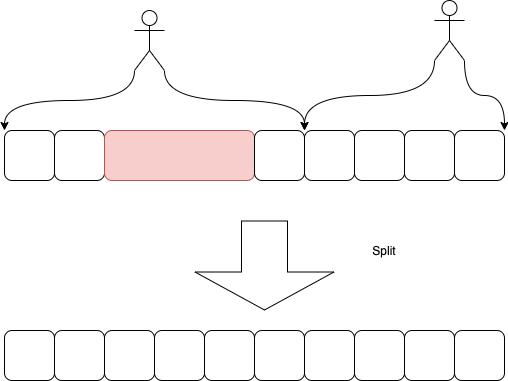
\includegraphics[width=0.7\textwidth]{loadbalance.png}
    \caption{负载均衡示意图}
    \label{负载均衡示意图}
\end{figure}

在后续测试中发现,随着矩阵规模的扩大,负载均衡算法会遇到内存带宽的瓶颈,导致由负载均衡的消耗远大于使用负载均衡带来的性能优化。对于这个问题本文提出了两种解决方案:一是利用NUMA架构的特性,提升内存带宽;而是在预处理阶段统计每个任务的计算任务负载情况的最大值和最小值。只对两者差距不是很大就不进行负载均衡。


\section{使用SIMD指令}

并行SpTRSV算法的第二个循环可以通过SIMD指令进行优化。由于ARM Neon只提供了128bit的向量寄存器,只能放下两个double和四个float,这里只对float类型的数据进行向量化计算的操作。算法流程为:首先用数据类型float32x\_t创建两个Neon寄存器变量vec\_xi、vec\_csaVal,该数据类型表示一个向量中有4个float32数据,分别表示由行号为i的未知数x组成的向量和稀疏矩阵一列上非零元组成的向量。将原来步长为1的循环,现在要修改为步长为4的循环。然后使用vld1q\_f32指令将稀疏矩阵中的4个非零元load进入vec\_csaVal寄存器当中,使用vld1q\_dup\_f32,将xi复制4份,load进vec\_xi寄存器中。之后使用vmulq\_f32,执行向量乘法的操作。最后使用vgetq\_lane\_f32(vec\_result),将向量乘法的结果从寄存器中取出,并写会内存当中。

在将结果写会内存的时候,由于一列上的非零元的行号都是离散的,因此对应产生结果的行号也不是连续的,这就导致本文们无法通过一个store命令直接将结果写如left\_sum中,而是需要分开进行独立的写操作。

\begin{lstlisting}[caption={SIMD指令优化}]
    float32x4_t vec_xi;
    float32x4_t vec_csaVal;
    vec_xi = vld1q_dup_f32(&xi);
    for each nonzero in column (step_size = 4) {
        result[0] = vgetq_lane_f32(vec_csaVal, 0);
        result[1] = vgetq_lane_f32(vec_csaVal, 1);
        result[2] = vgetq_lane_f32(vec_csaVal, 2);
        result[3] = vgetq_lane_f32(vec_csaVal, 3);
        STORE result;
    }
\end{lstlisting}

\section{使用LSE指令}

由于算法使用了大量的原子操作,例如对于left\_sum和in\_degree使用了很多的原子操作,使用原有争抢式的原子指令会对程序的性能产生消极影响。在开启LSE原子指令之前CAS操作需要通过LDXR和STXR并通过不断判断的方式实现,而在开启LSE只需一条casal指令,同样原子加法操作也只需一条LDADD指令。

具体实现方式为,通过编译器参数'-march=armv8-a+lse'来实现

\section{使用NUMA架构}

NUMA架构的优点是扩展了系统的内存带宽,提升了系统的CPU核心数目,缓解了缓存一致性的冲突。但是却带来了远程内存访问,延迟过高等缺陷。软件设计人员需要充分考虑并利用这个特性,否则会带来性能的损失。

通过numactl --hardware命令可以获得本机的numa硬件情况,本机使用的NUMA特性如图所示\ref{numaHardware}。从该图node distances可以看出远程访问的延迟可以为本地访问延迟的1.6至3.3倍。

\begin{figure}[htbp]
    \centering
    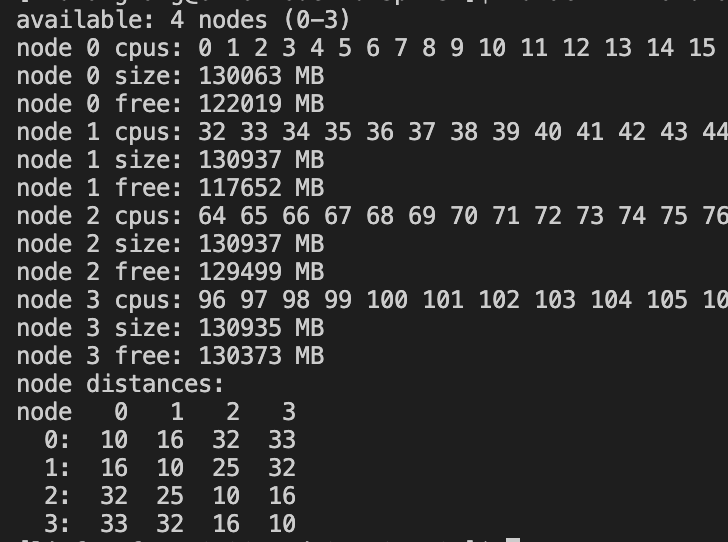
\includegraphics[width=0.7\textwidth]{numaHardware.png}
    \caption{本机所使用的硬件特性}
    \label{numaHardware}
\end{figure}

本算法使用的数据按照读写特征主要分为以下二类:
\begin{enumerate} \setlength{\itemsep}{0pt}
    \item 只读数据类型:稀疏的三个数组,cscCowPtr[]、cscRolIdx[]、cscVal[]以及等式$Lx=b$右边的向量b[]。
    \item 频繁通过原子操作读写:left\_sum[]、in\_degree[]、未知数向量x[]
\end{enumerate}

对于只读的数据类型本文主要通过创建数据副本的形式,将只读数据分成四分,分配到四个NUMA节点上。主要是通过通过Linux操作系统提供的C语言编程接口\cite{libnuma}libnuma中的void *numa\_alloc\_onnode(size\_t size, int node),接口参数int node表示指定结点的编号。线程首先通过sched\_getcpu()和numa\_node\_of\_cpu(cpuid),得到自己所在结点的信息,根据这个信息来访问局部数据。然而对于频繁通过原子操作读写的数据,由于数据读写的随机性,没法使用numa架构进行很好的优化。

总的来说,本文主要尝试了四种种NUMA策略。
\begin{enumerate} \setlength{\itemsep}{0pt}
    \item 使用numactl --cpunodebind,将所有任务都固定在一个结点上。
    \item 使用numactl --cpunodebind,将任务固定在两个距离相近的NUMA节点上。
    \item 使用numactl --interleave,将数据均匀分布在四个numa节点上。
    \item 创建只读数据副本,并将其分配到各个结点上。
\end{enumerate}

经过测试发现对于小规模或者并行性第的稀疏矩阵固定在单一结点上性能是最好的。而对于规模较大并行性较好的稀疏矩阵,我采用策略4,也就是创建只读数据副本,并将数据与任务分配到多个节点上能获得约15\%的性能提升,详见\ref{NUMA架构对性能的影响}

\section{本章总结}

本章介绍了本文所提出的SpTRSV算法的设计以及优化思路。包括一些程序读入,数据整理以及结果验证的辅助操作,基本的并行架构及其在此基础上的优化技巧。主要的优化技巧有:通过prefetch指令进行预缓存;使用CPU松弛技术提升自旋等待的整体性能;使用padding的方法消除伪共享;在分析矩阵任务负载不均衡的基础上提出了负载均衡的策略;使用SIMD指令进行优化;通过编译指令的方式开启LSE指令集,优化了原子操作的性能;以及针对NUMA架构进行了一系列的策略尝试优化。


\endinput
\chapter{实验结果分析}
\section{算法总体性能测试}

本次测试所用的矩阵主要来自于\cite{park2014sparsifying}和\cite{liuSyncFree2016}这两篇文章中所用到的矩阵,这些矩阵都可以从MatrixMarket和弗罗里达大学稀疏矩阵集合中下载。本次测试所使用的矩阵如表\ref{MatrixSuite}所示。表中最后一列并行性的定义为并行性=矩阵的行数$ \div $最大level数,可以理解为平均每个level有多少的任务即可,其中并行性最好的是矩阵是nlpkkt160,只有两个level,理论并行性最差的是af\_shell10和chipcool0。

\begin{table}[htbp]
    \scriptsize
    \caption{性能测试所用矩阵}
    \label{MatrixSuite}
    \resizebox{\textwidth}{!}{%
    \begin{tabular}{|l|r|r|r|r|}
    \hline
    矩阵名称 & 行或列数量 & 非零元个数 & 最大level数 & 并行性 \\ \hline
    nlpkkt160     & 8,345,600     & 229,518,112   & 2   & 4,172,800   \\
    road\_usa     & 23,947,347    & 57,708,624    & 77  & 311,004     \\
    road\_central & 14,081,816    & 33,866,826    & 59  & 238,674     \\
    wiki-Talk     & 2,394,385     & 5,021,410     & 522 & 4,586       \\
    webbase-1M    & 1,000,005     & 3,105,536     & 514 & 1,945       \\
    apache2       & 715,176       & 4,817,870     & 664 & 1,077       \\
    thermal2      & 1,228,045     & 8,580,313    & 1,239& 991        \\
    G3\_circuit   & 1,585,478     & 7,660,826    & 2,594& 611         \\
    StocF-1465    & 1,465,137     & 21,005,389   & 3,004& 487         \\
    af\_shell10   & 1,508,065     & 52,259,885   & 8,360& 180         \\
    chipcool0     & 20,082        & 2,81,150     & 534  & 37          \\ \hline
    \end{tabular}%
    }
\end{table}

实验所用的硬件平台为华为鲲鹏920处理器,4个NUMA结点,每个结点有32个核心以及130GB的内存,结点间带宽为480Gbps。软件平台:操作系统CentOS7.6.1810。编译器gcc9.0。openmp4.5。

首先,图\ref{在多个稀疏矩阵上的测试数据}展示了在11个稀疏矩阵下的性能测试数据,绝大多数的矩阵都能够获得2倍以上的加速比(黄色那条线)。折线图的横坐标为矩阵的名称,按照表\ref{MatrixSuite}中,矩阵的并行性从高到低排序。可以看出,矩阵并行性越高,加速比越高。

\begin{figure}[htbp]
    \centering
    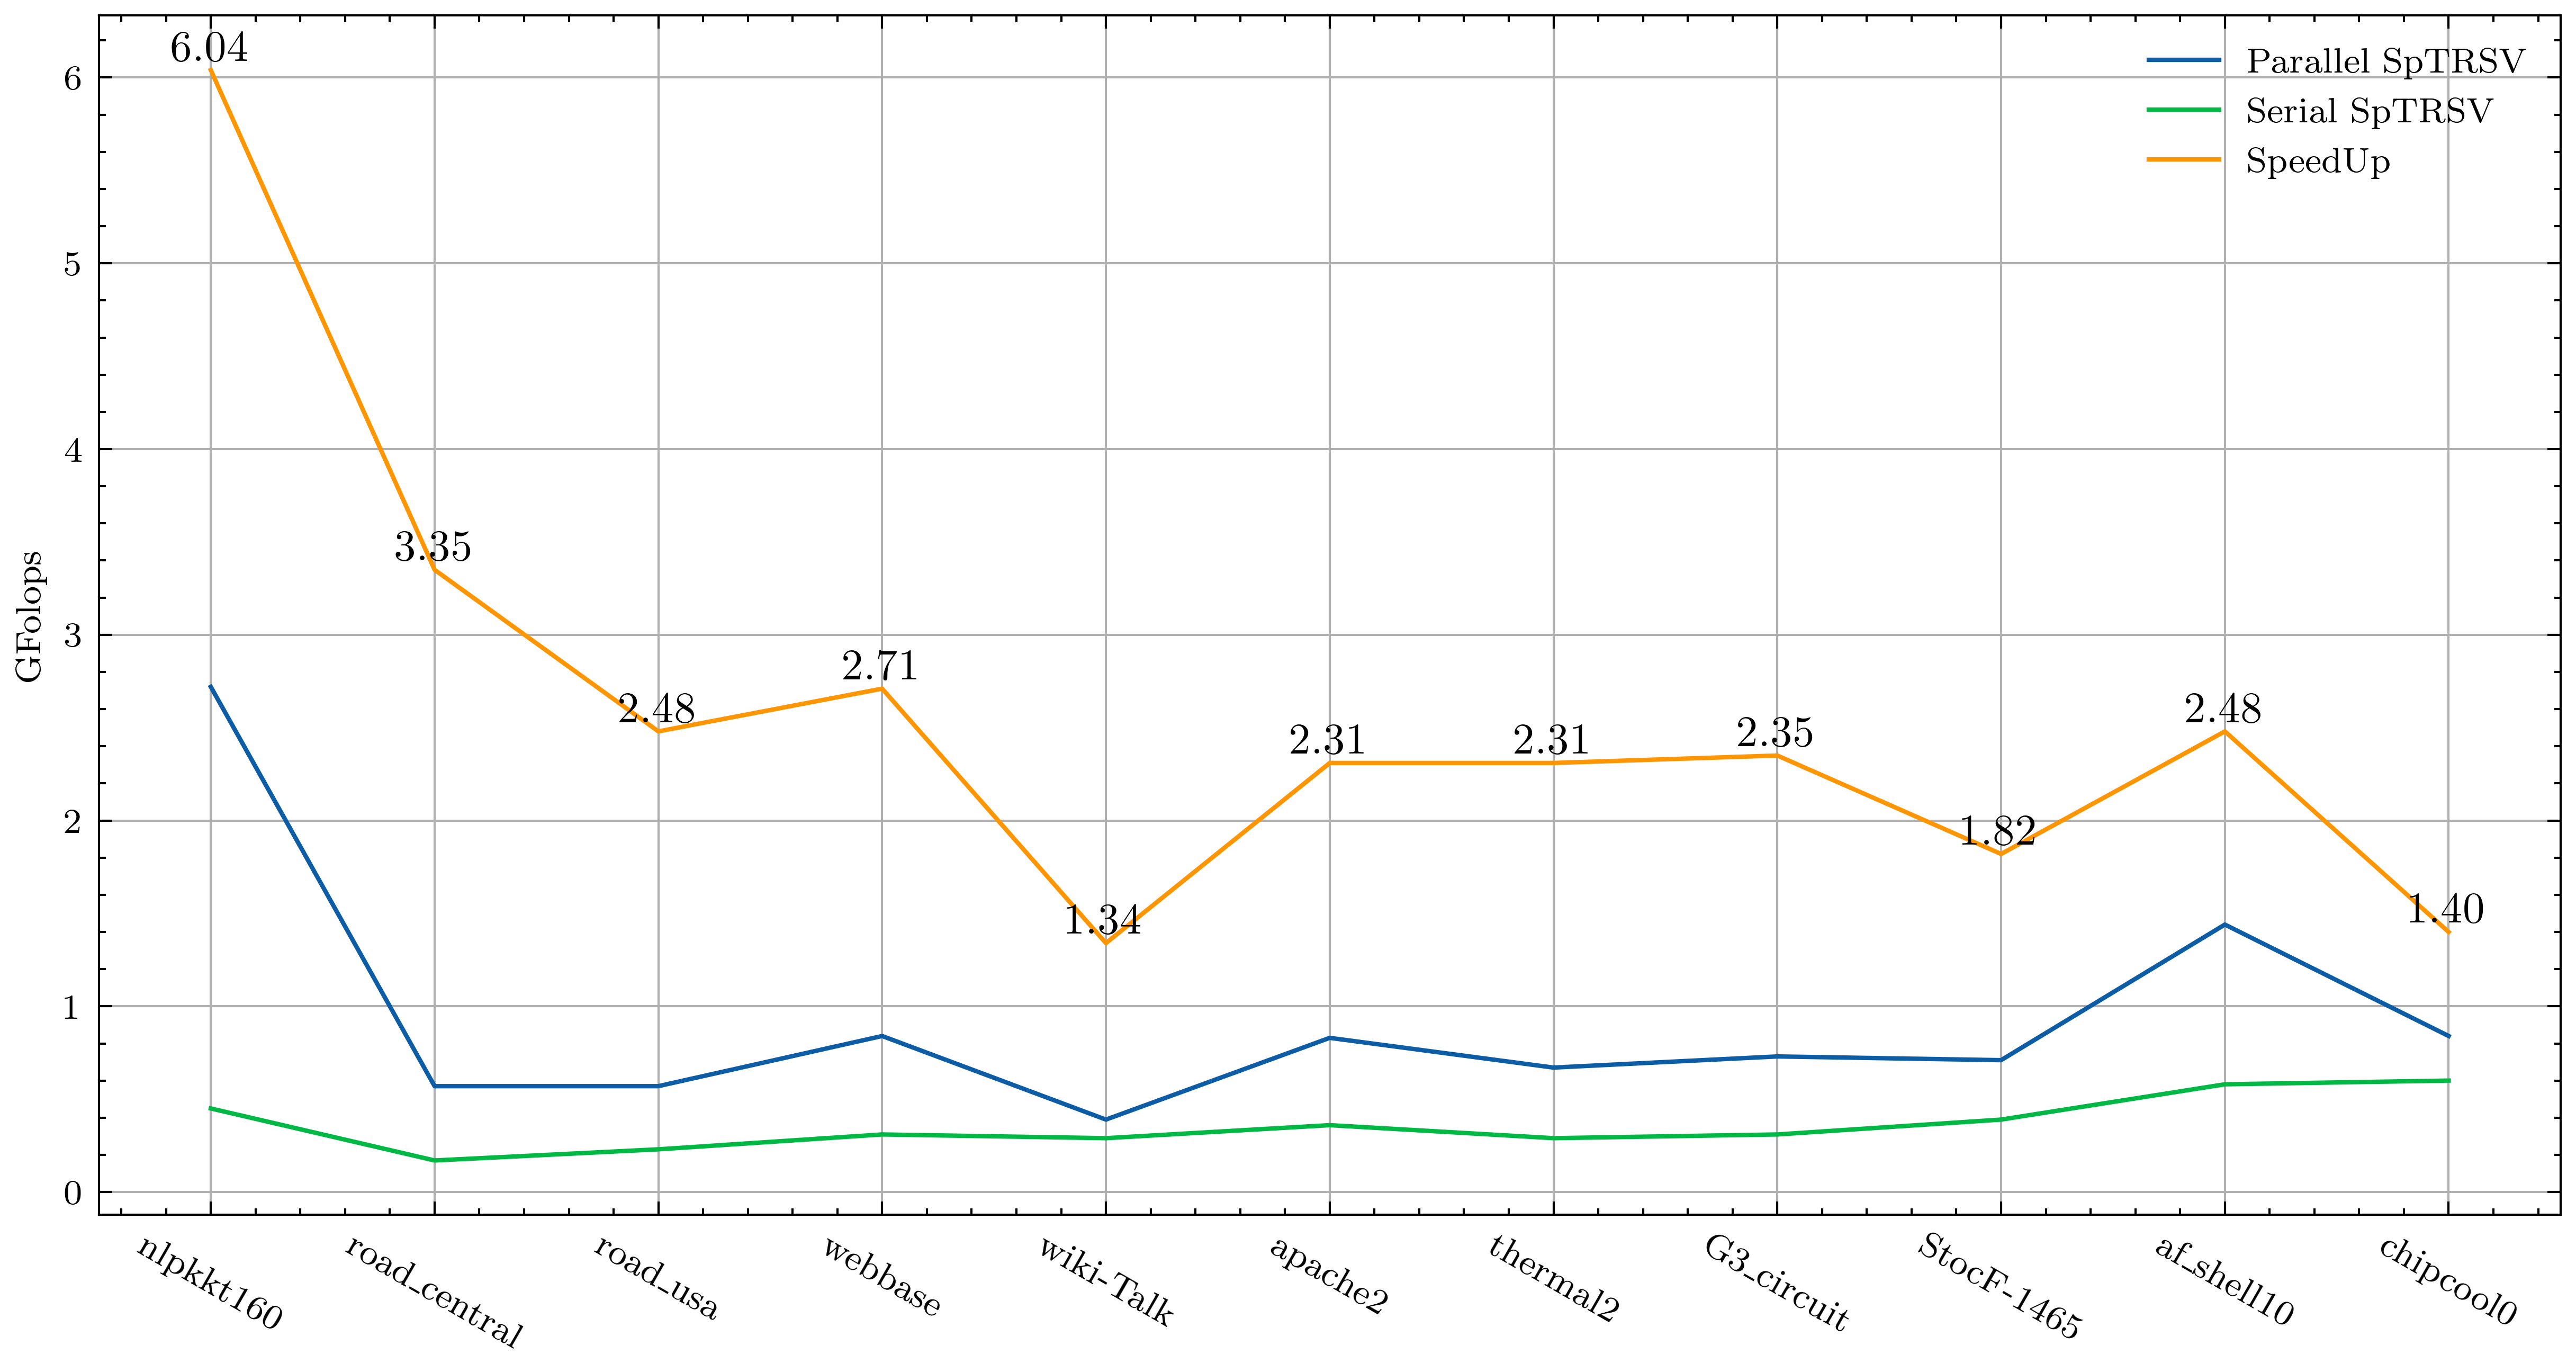
\includegraphics[width=0.9\textwidth]{moreData.png}
    \caption{在多个稀疏矩阵上的测试数据}
    \label{在多个稀疏矩阵上的测试数据}
\end{figure}

~\\

% 然后,将本文提出的SpTRSV算法与intel MKL数学库中的SpTRSV算法进行了性能对比,结果如图\ref{SpTRSVMulti-paltform}所示,intel平台采用CPU双路志强E5-2695v3 14x2个核心,130GB内存,MKL版本为11.3。柱状图从左到右依次为:MKL数学库中串行算法的性能、并行算法的性能;在鲲鹏920处理器上,使用本文提出的串行算法的性能、并行算法的性能;纵轴以Gflops为单位来衡量算法的性能。Gflops计算方法为$(2 \times NNZL)  \div totoal\_time$。$totoal\_time = preprocess\_time + calculate\_time$。NNZL表示下三角矩阵非零元的个数,采用双精度浮点类型,所以前面乘2。6张图分别对应6个稀疏矩阵。

% 可以看出,对于并行性较好的矩阵,如nlpkkt160和road\_central,并行算法取得了相比于串性算法3倍以上的加速比。而对于那些并行性较差的矩阵如wiki-Talk以及chipcool0,由于level数量较多,能够获得有限的加速比。

% \begin{figure}[htbp]
%     \centering
%     \subfigure{
%     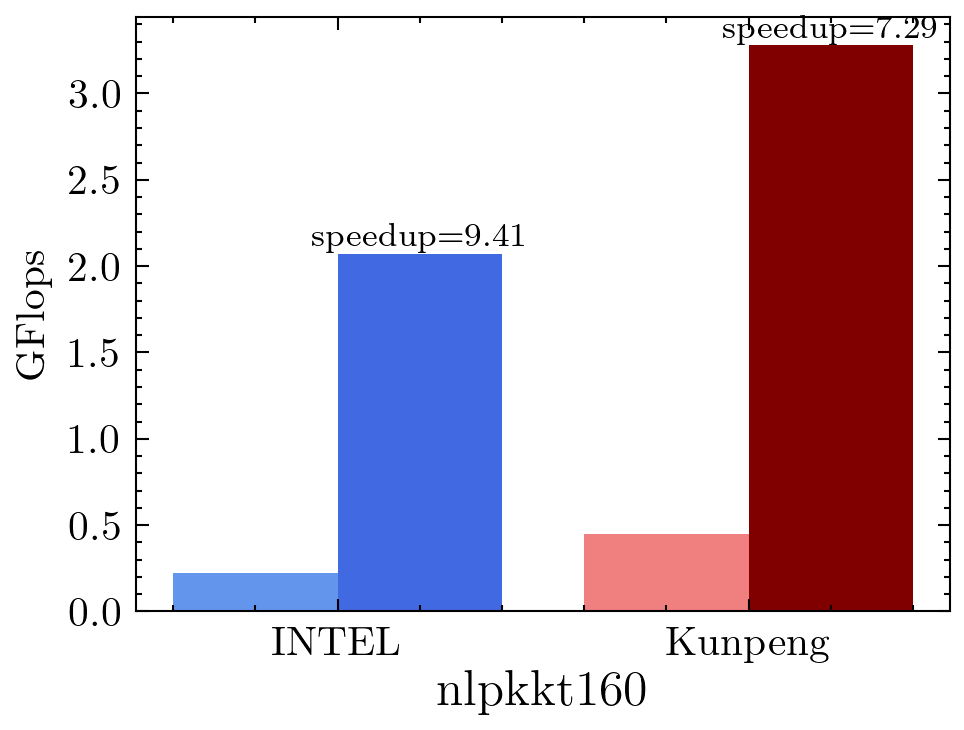
\includegraphics[width=6.5cm]{result0.png}
%     }
%     \quad
%     \subfigure{
%     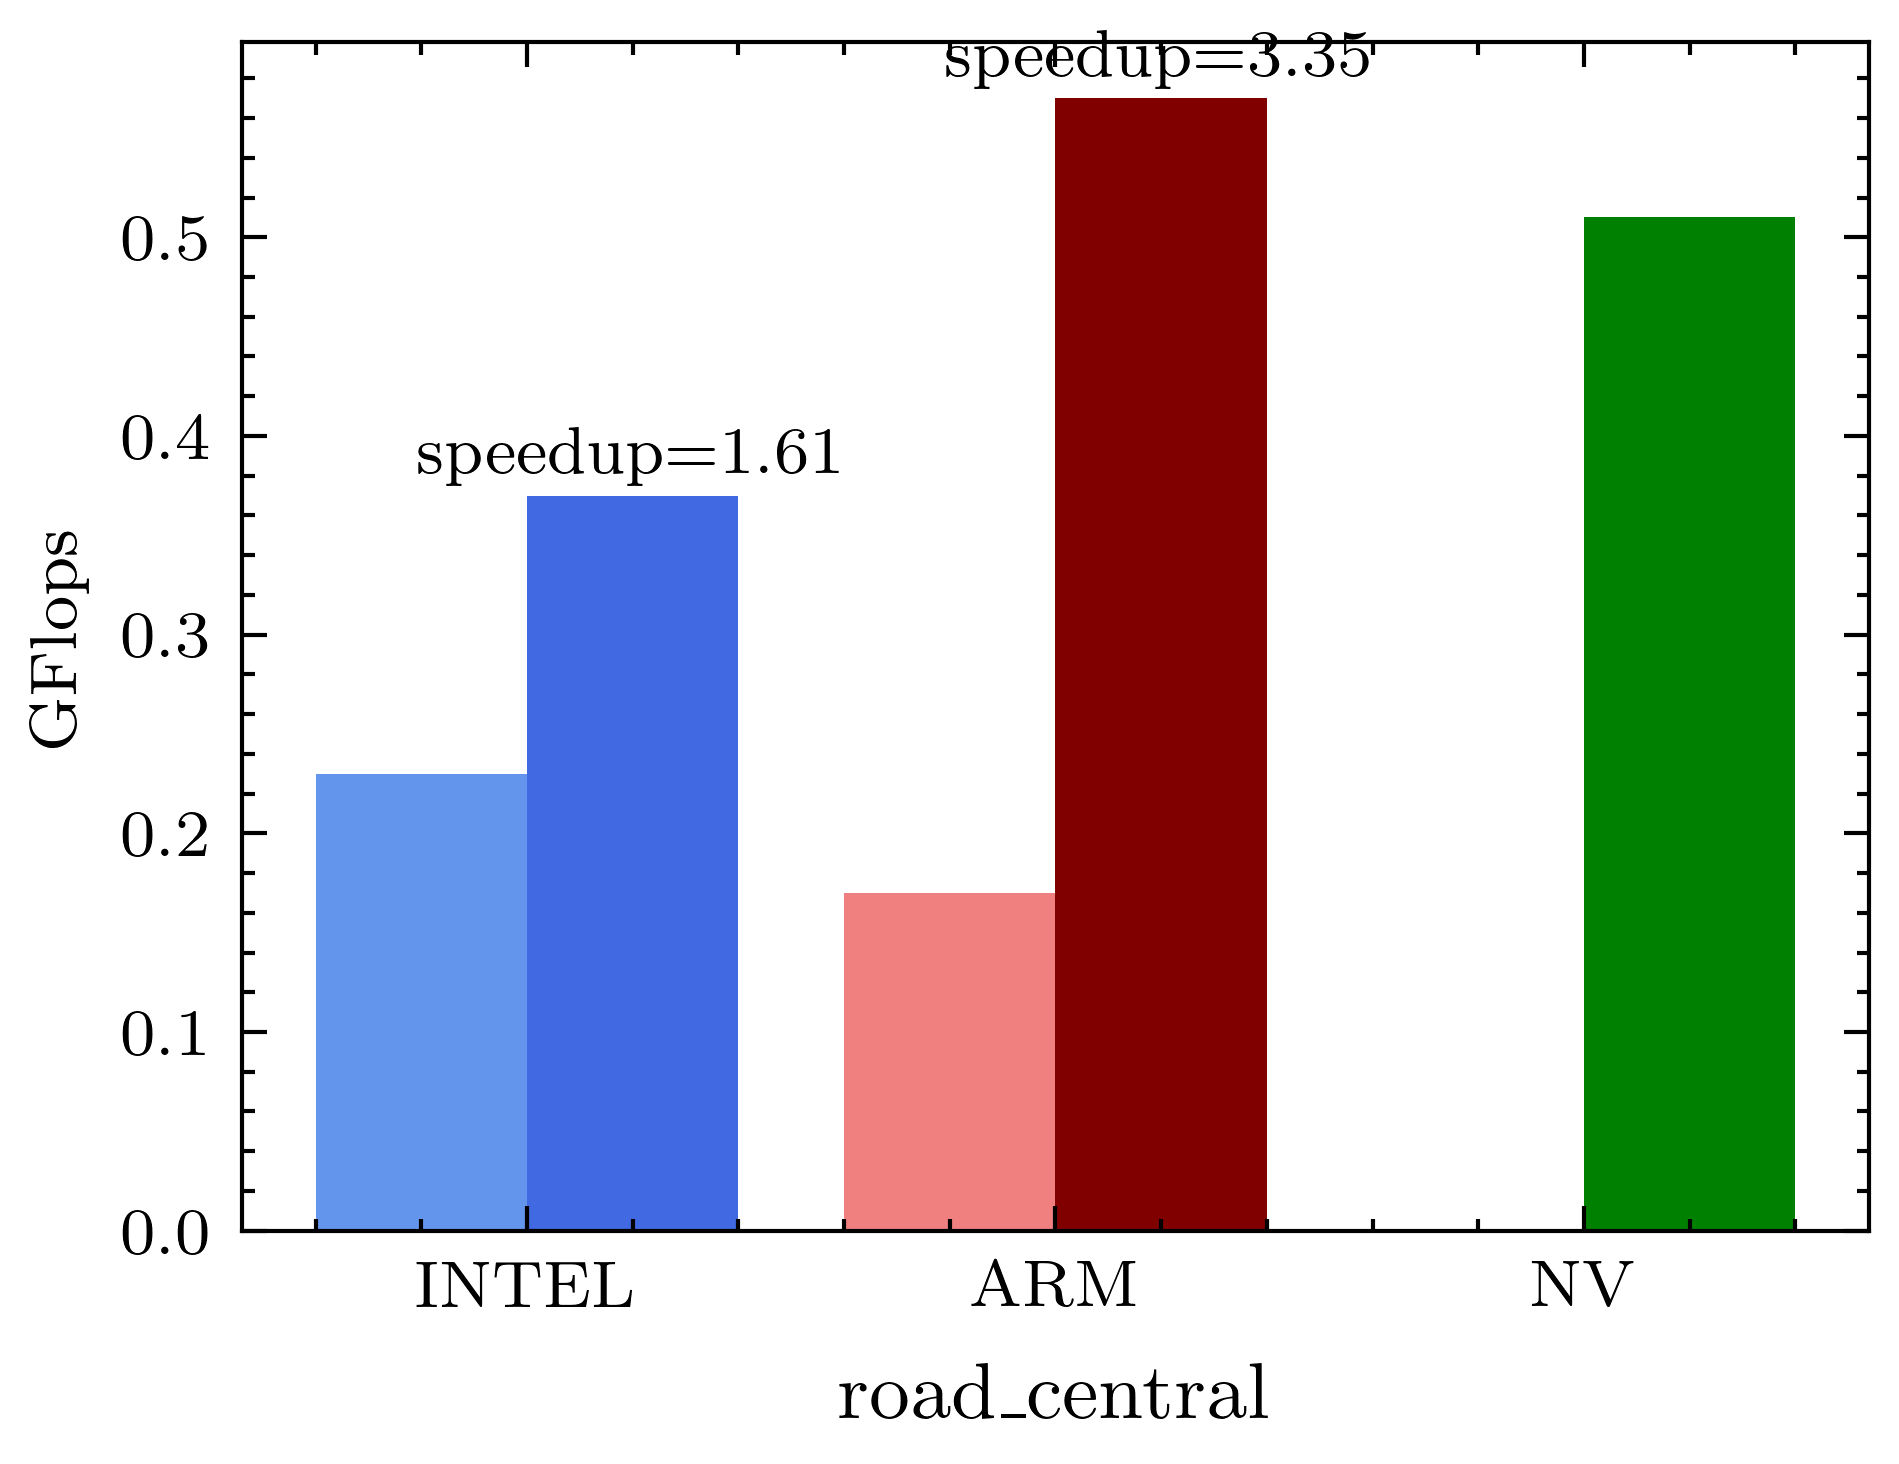
\includegraphics[width=6.5cm]{result1.png}
%     }
%     \quad
%     \subfigure{
%     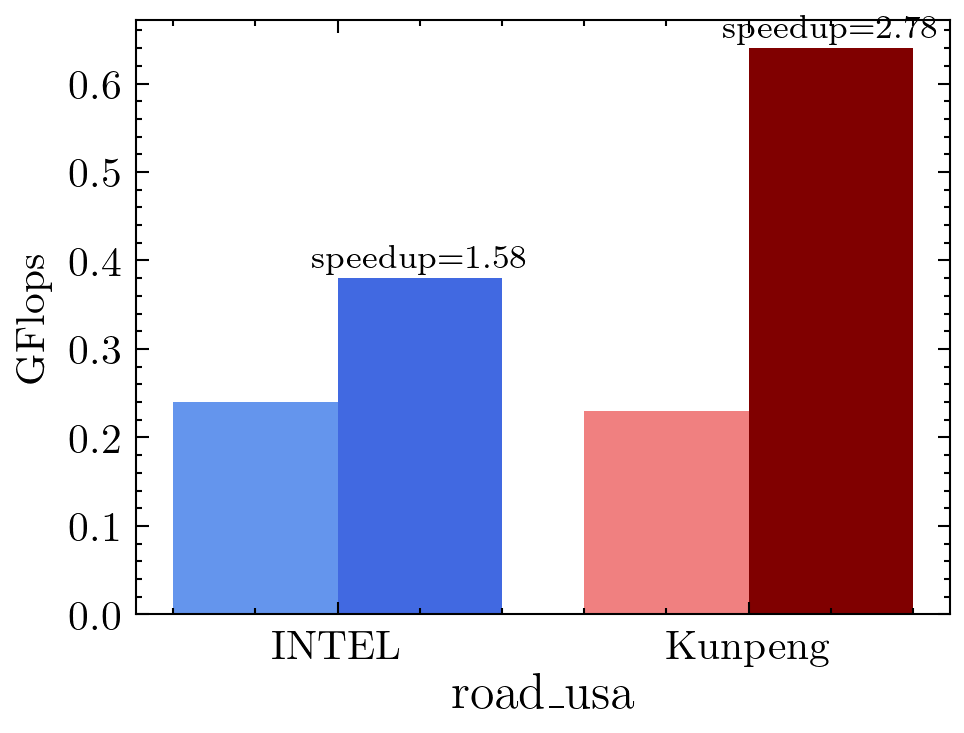
\includegraphics[width=6.5cm]{result2.png}
%     }
%     \quad
%     \subfigure{
%     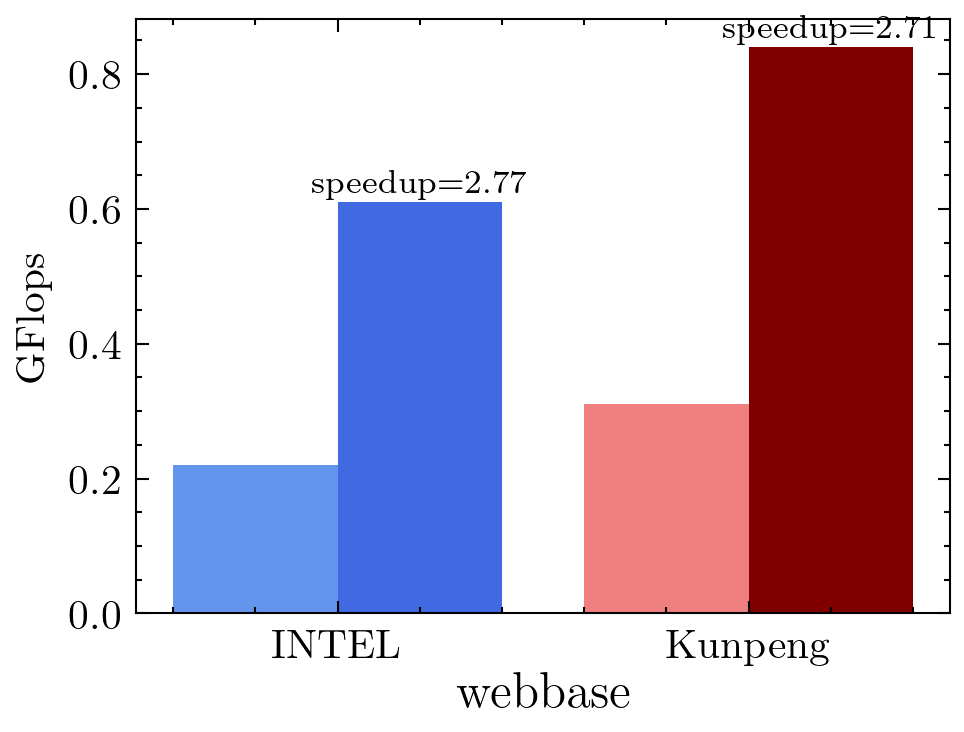
\includegraphics[width=6.5cm]{result3.png}
%     }
%     \quad
%     \subfigure{
%     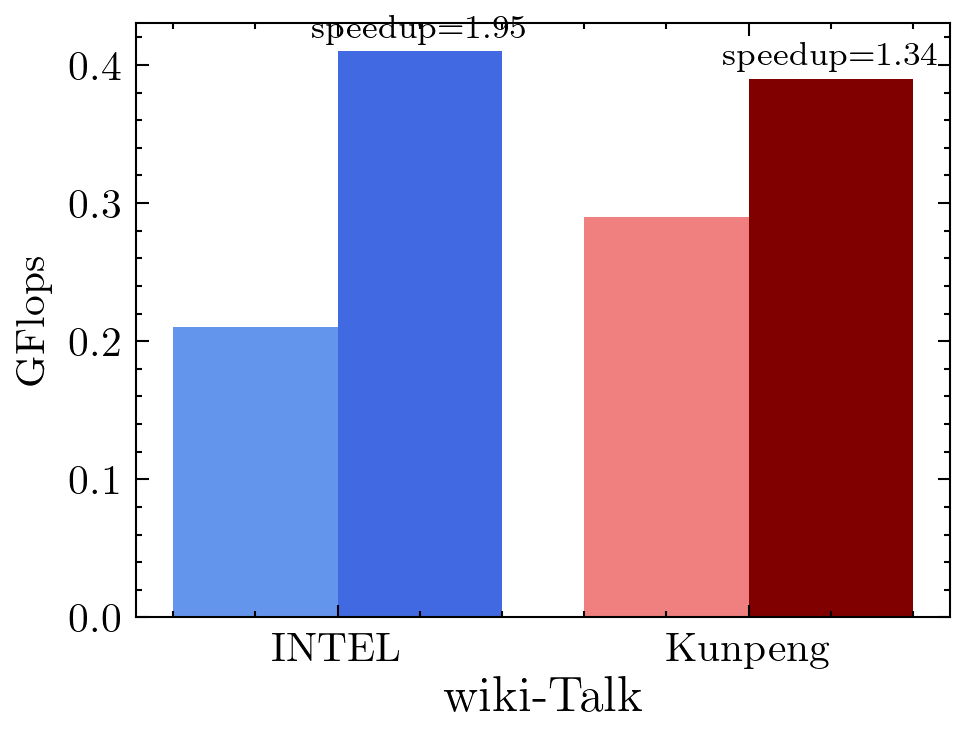
\includegraphics[width=6.5cm]{result4.png}
%     }
%     \quad
%     \subfigure{
%     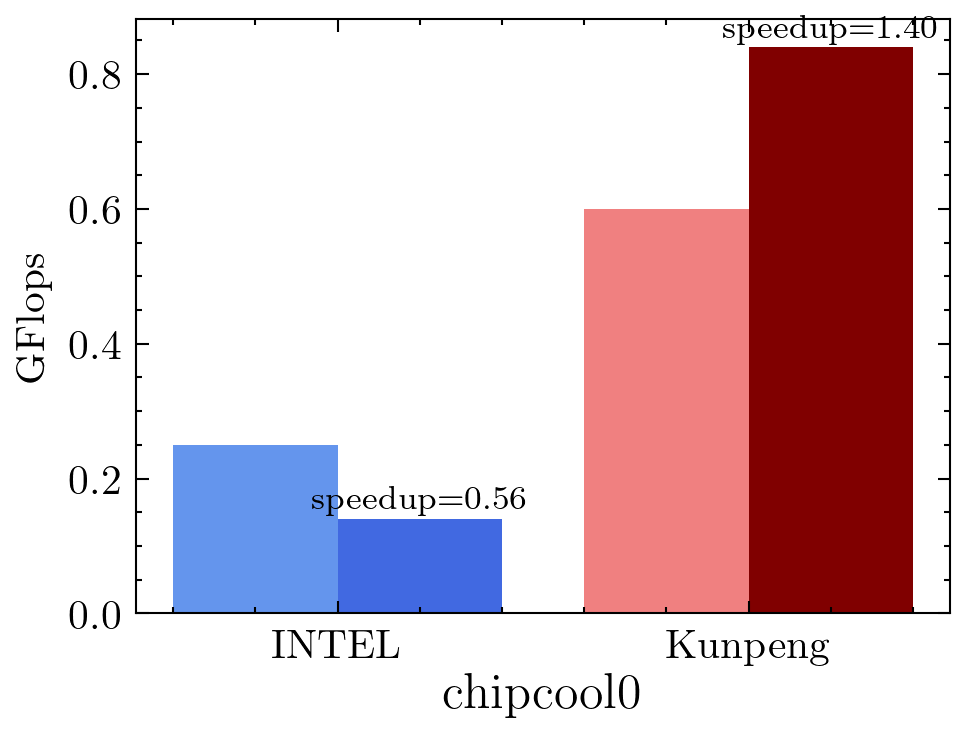
\includegraphics[width=6.5cm]{result5.png}
%     }
%     \caption{本文算法与intel MKL中算法的性能对比}
%     \label{SpTRSVMulti-paltform}
% \end{figure}

\begin{table}[htbp]
    \scriptsize
    \caption{算法耗时分解表}
    \label{算法耗时分解表}
    \resizebox{\textwidth}{!}{%
    \begin{tabular}{|l|r|r|r|r|}
    \hline
    矩阵名称         & 预处理时间(ms) & 计算消耗时间(ms) & 总时间(ms) & 预处理时间占总时间的比例 \\ \hline
    nlpkkt160    & 18.70 & 68.68  & 87.38   & 21.4\%       \\
    road\_central & 20.85 & 87.76  & 108.61  & 19.1\%       \\
    road\_usa     & 42.08 & 141.9  & 77      & 22.8\%       \\
    webbase-1M   & 1.30  & 4.29   & 514     & 23.2\%       \\
    wiki-Talk    & 3.82  & 13.91  & 522     & 21.5\%       \\
    chipcool0    & 0.12  & 0.24   & 534     & 33.3\%       \\ \hline
    \end{tabular}%
    }
\end{table}

如表\ref{算法耗时分解表}所示,算法在预处理阶段主要进行in\_degree的计算,以及通过任务划分的方式进行负载均衡的处理。预处理时间占总时间的20\%左右,且相对稳定。而且,相比于J.Park\cite{park2014sparsifying}基于level-sets的算法(表\ref{任务耗时分解图}),本文的算法在预处理阶的时间消耗很少,例如对于矩阵nlpkkt,基于level-sets的算法需要484.07ms的时间,而本文的算法只需要18.70ms的预处理时间,以及68.68ms的计算时间。


\section{使用负载均衡对性能的提升}

图\ref{测试负载均衡对SpTRSV算法性能的影响}展示了负载均衡操作对算法性能的影响。对于一些任务之间负载相对均衡的矩阵如nlpkkt160,road\_central和road\_usa,负载均衡优化的开启和关闭,并没有很大的影响,相反对于webbase和chipcool,这两个矩阵之间存在着负载不均衡的现象,所以启用负载均衡起到了优化的作用。

\begin{figure}[htbp]
    \centering
    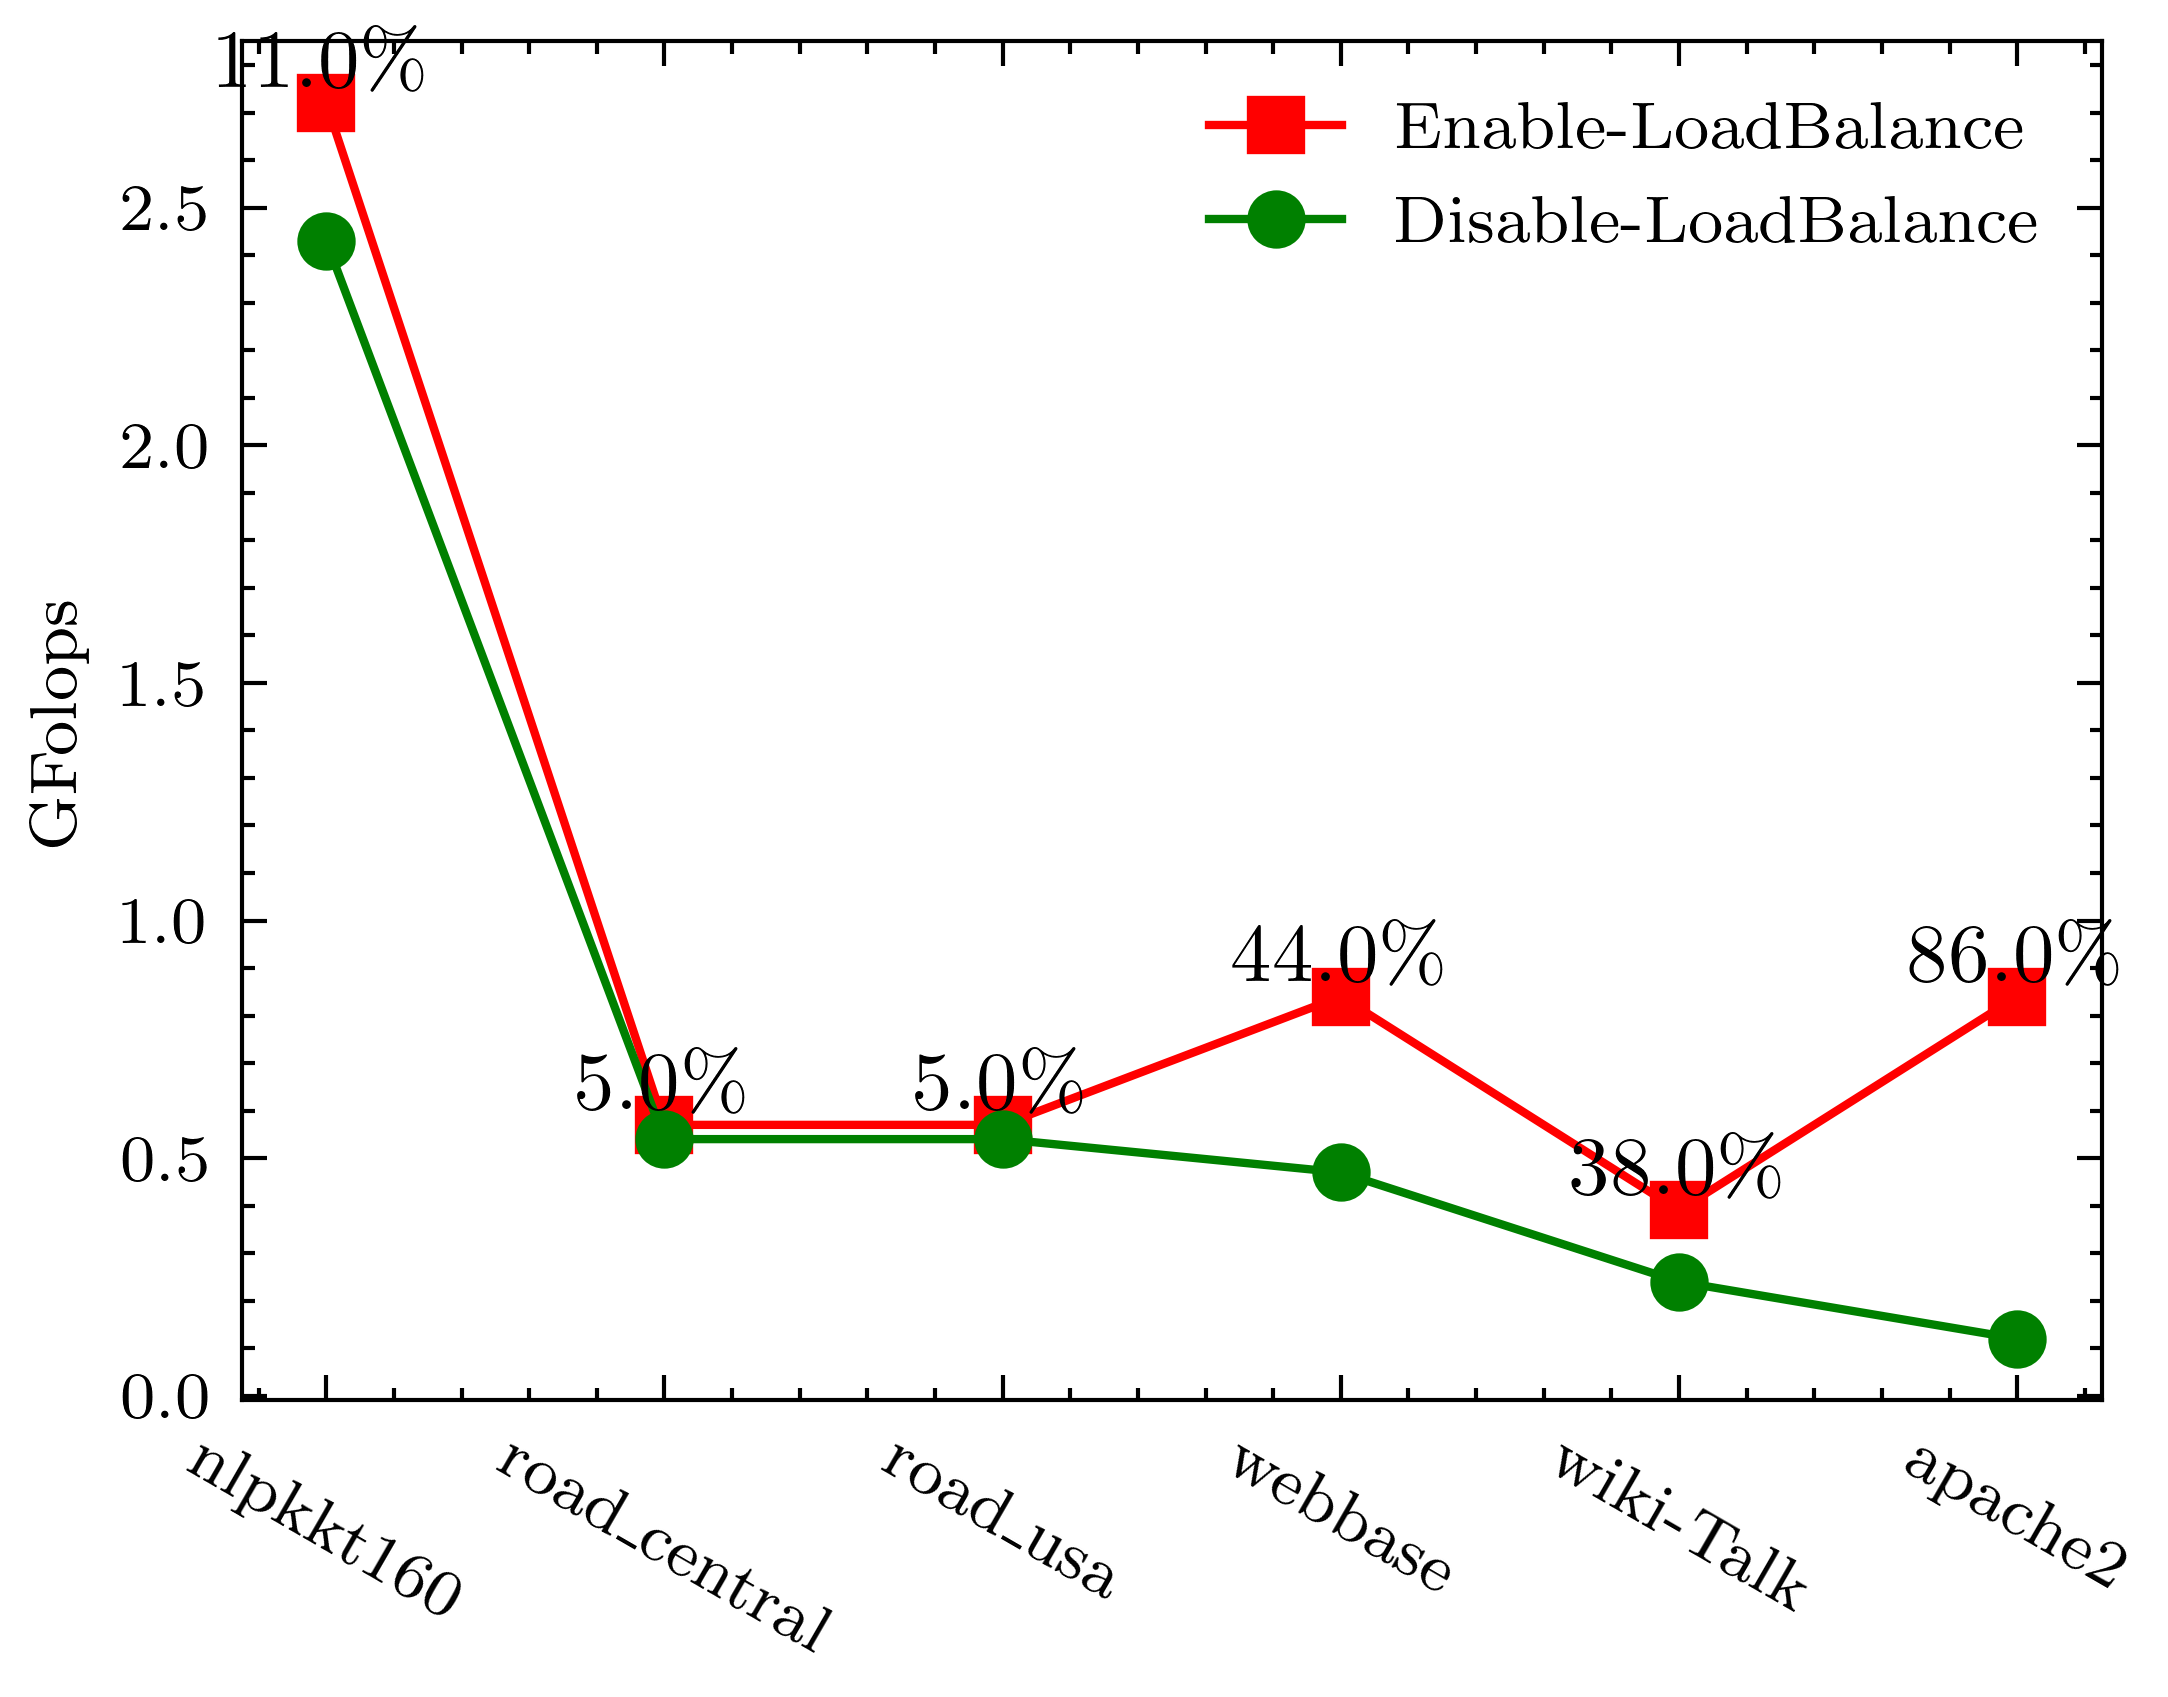
\includegraphics[width=0.7\textwidth]{lbtest.png}
    \caption{测试负载均衡对SpTRSV算法性能的影响}
    \label{测试负载均衡对SpTRSV算法性能的影响}
\end{figure}

\section{使用CPU松弛技术对性能的提升}

\begin{figure}[htbp]
    \centering
    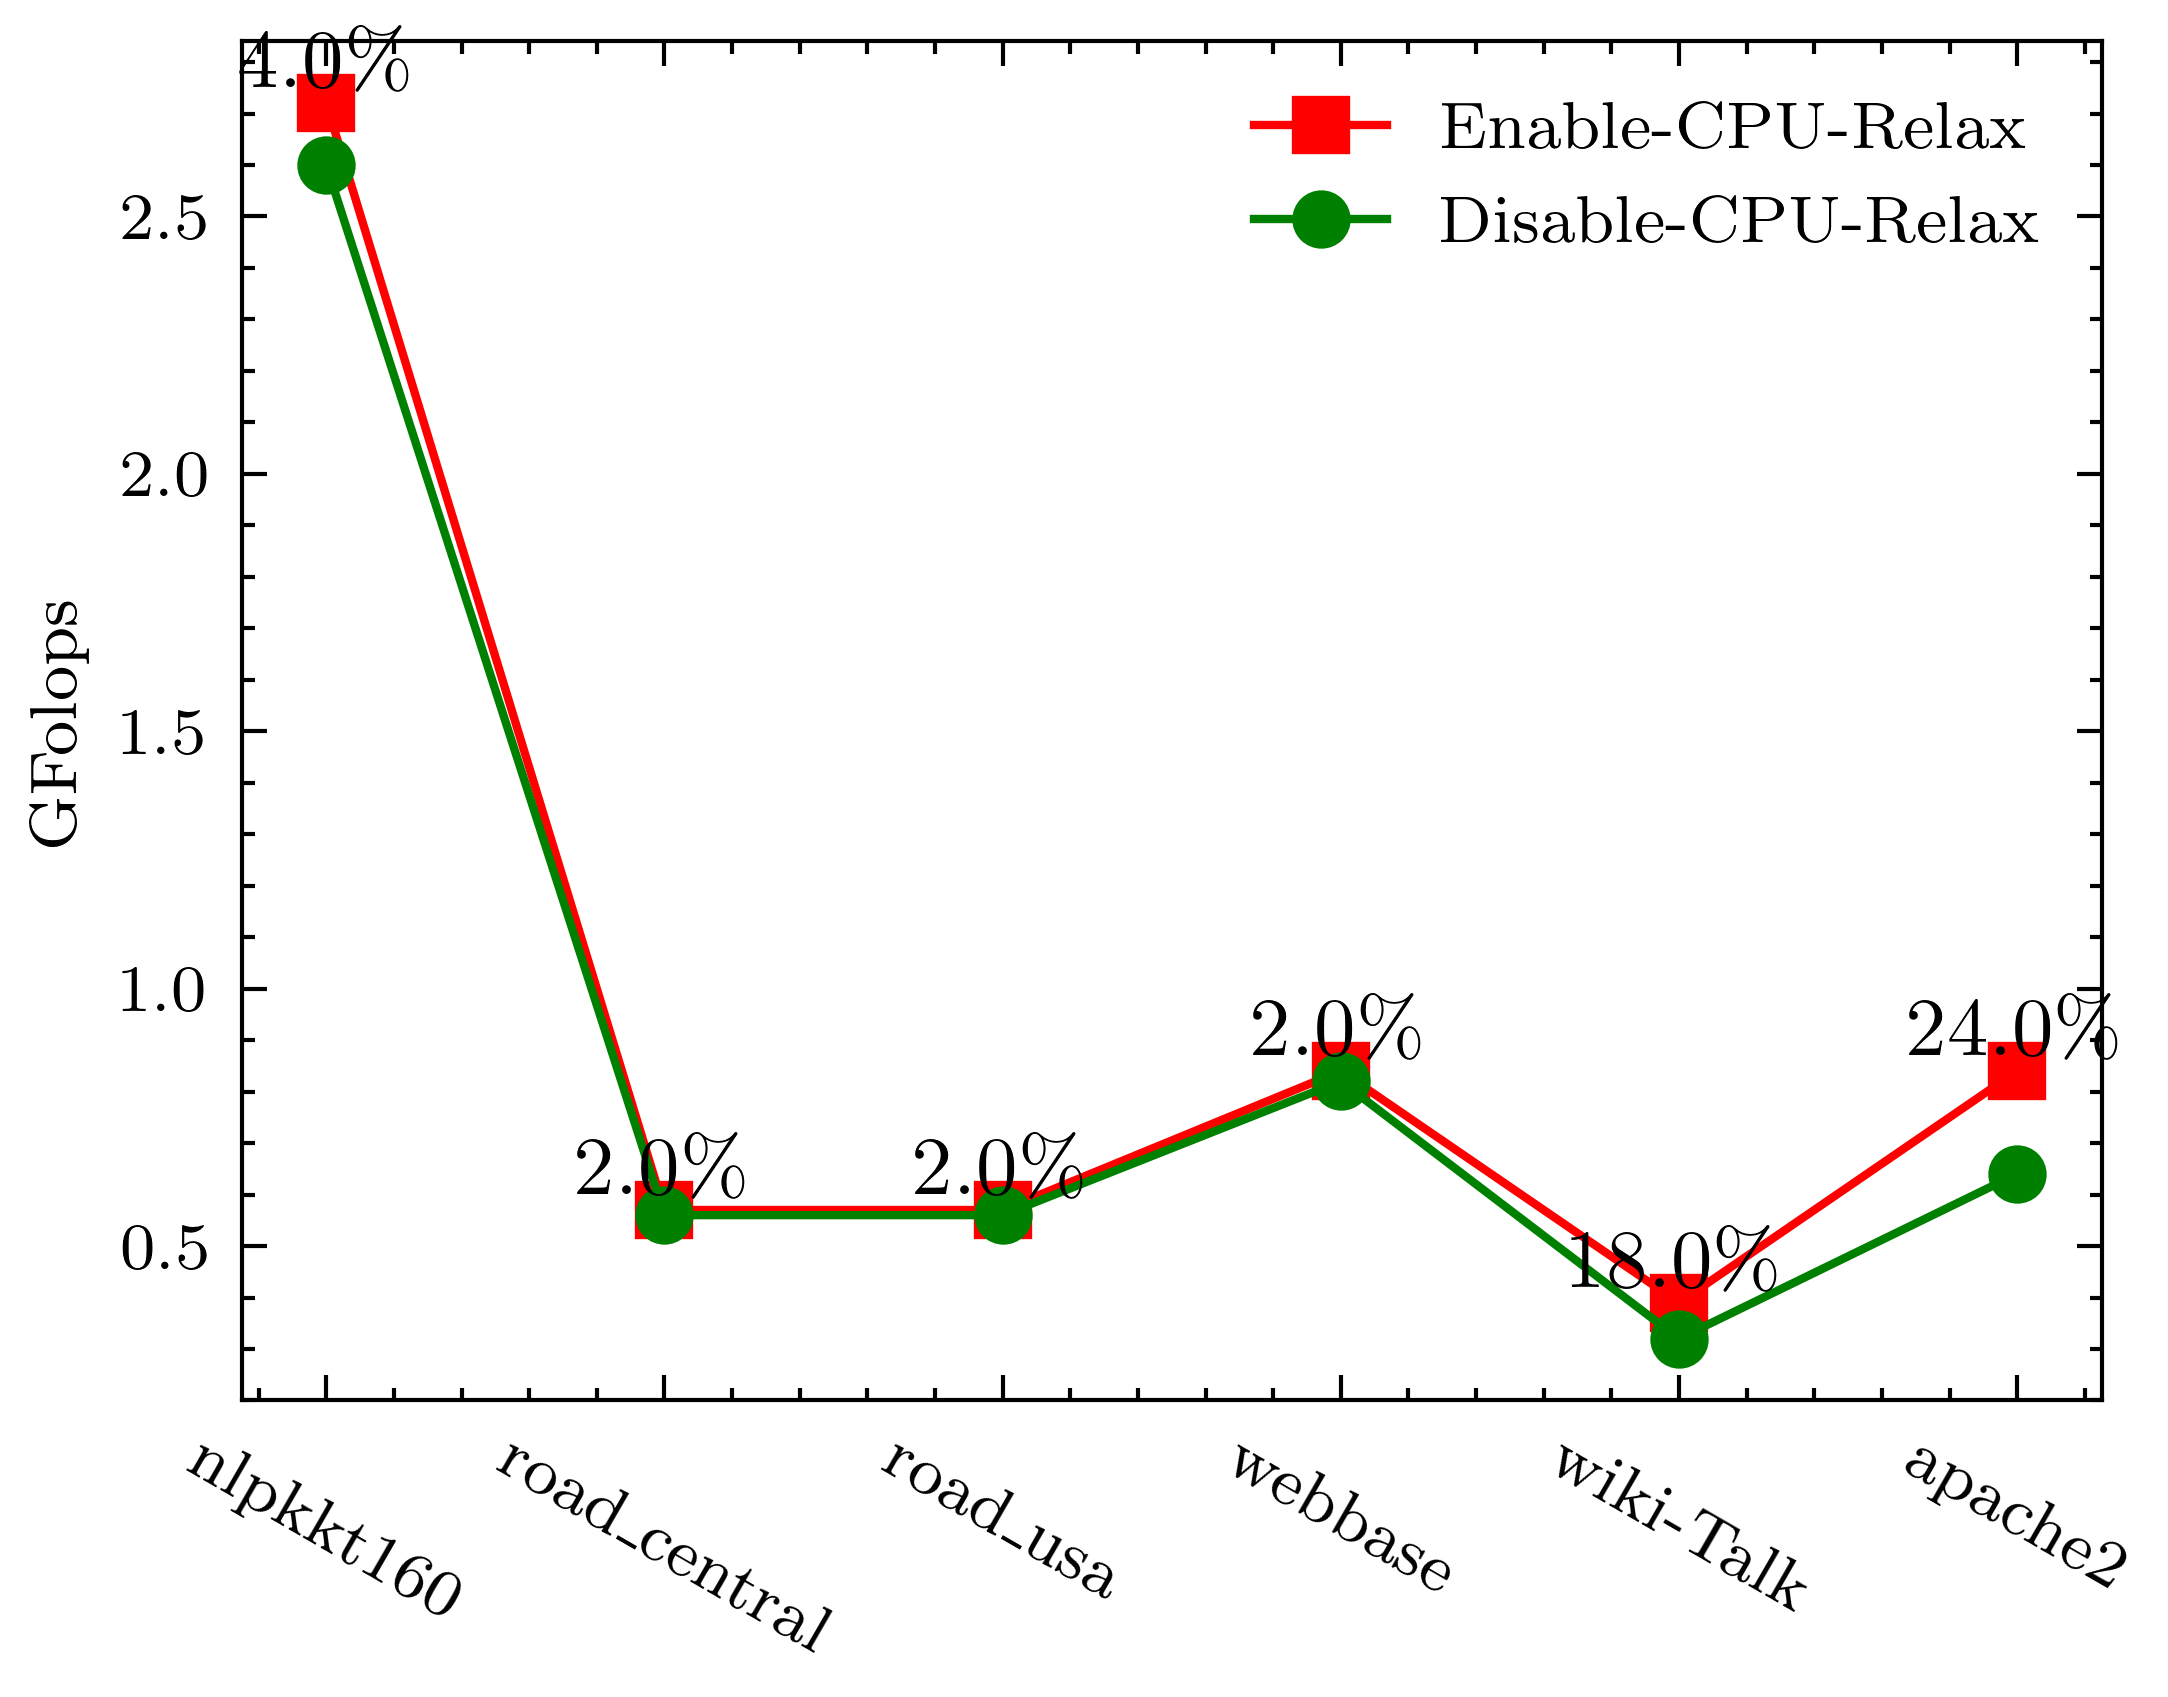
\includegraphics[width=0.7\textwidth]{cpuRelaxTest.png}
    \caption{测试CPU松弛技术对性能的影响}
    \label{测试CPU松弛技术对性能的影响}
\end{figure}

图\ref{测试CPU松弛技术对性能的影响}展示了CPU松弛技术对性能的影响。CPU松弛技术对于一些并行度相对较低的稀疏矩阵有一定的性能提升,总体来说对性能地提升相对较低。

\section{使用ARMv8原子指令对性能的提升}

\begin{figure}[htbp]
    \centering
    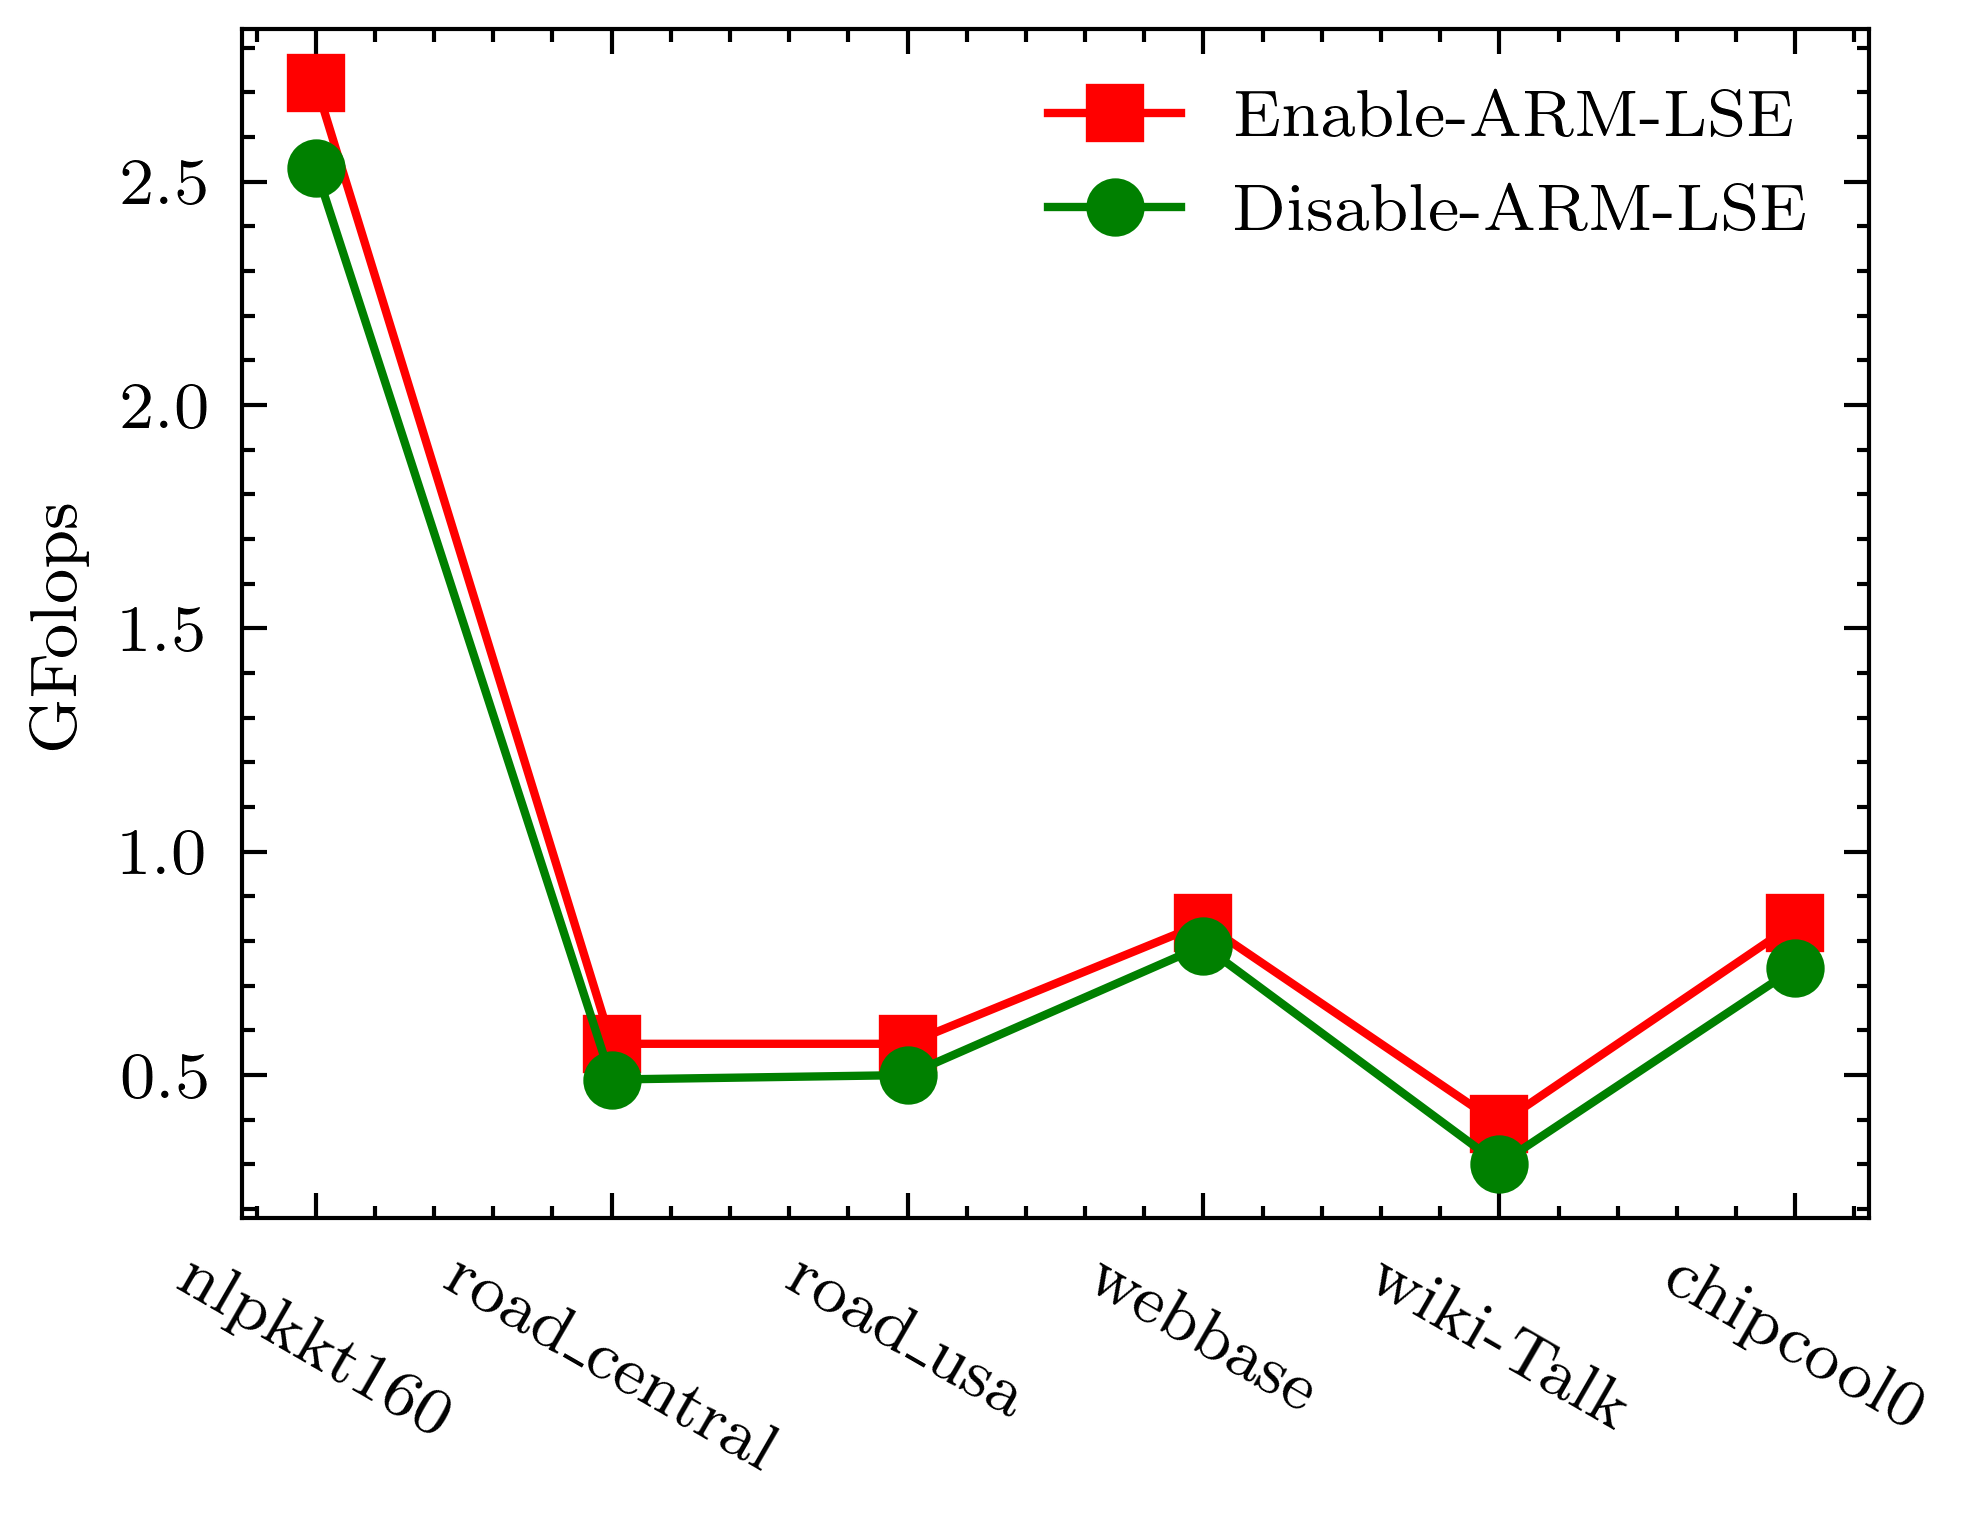
\includegraphics[width=0.7\textwidth]{ARMLSETEST.png}
    \caption{测试ARMv8原子指令对性能的影响}
    \label{测试ARMv8原子指令对性能的影响}
\end{figure}

图\ref{测试ARMv8原子指令对性能的影响}展示了ARMv8原子指令对算法性能的影响。在使用了ARMv8原子指令之后,性能相比于ARM传统的原子指令,性能有所提升。

\section{NUMA架构对性能的影响}\label{NUMA架构对性能的影响}

对于绝大多数的矩阵使用numctl命令将计算放到结点的内部,计算效率是最高的。但是对于规模较大,并行性较好的矩阵,将任务分配到两个NUMA结点上相比于单节点能够获得约10\%的性能提升。

\begin{figure}[htbp]
    \centering
    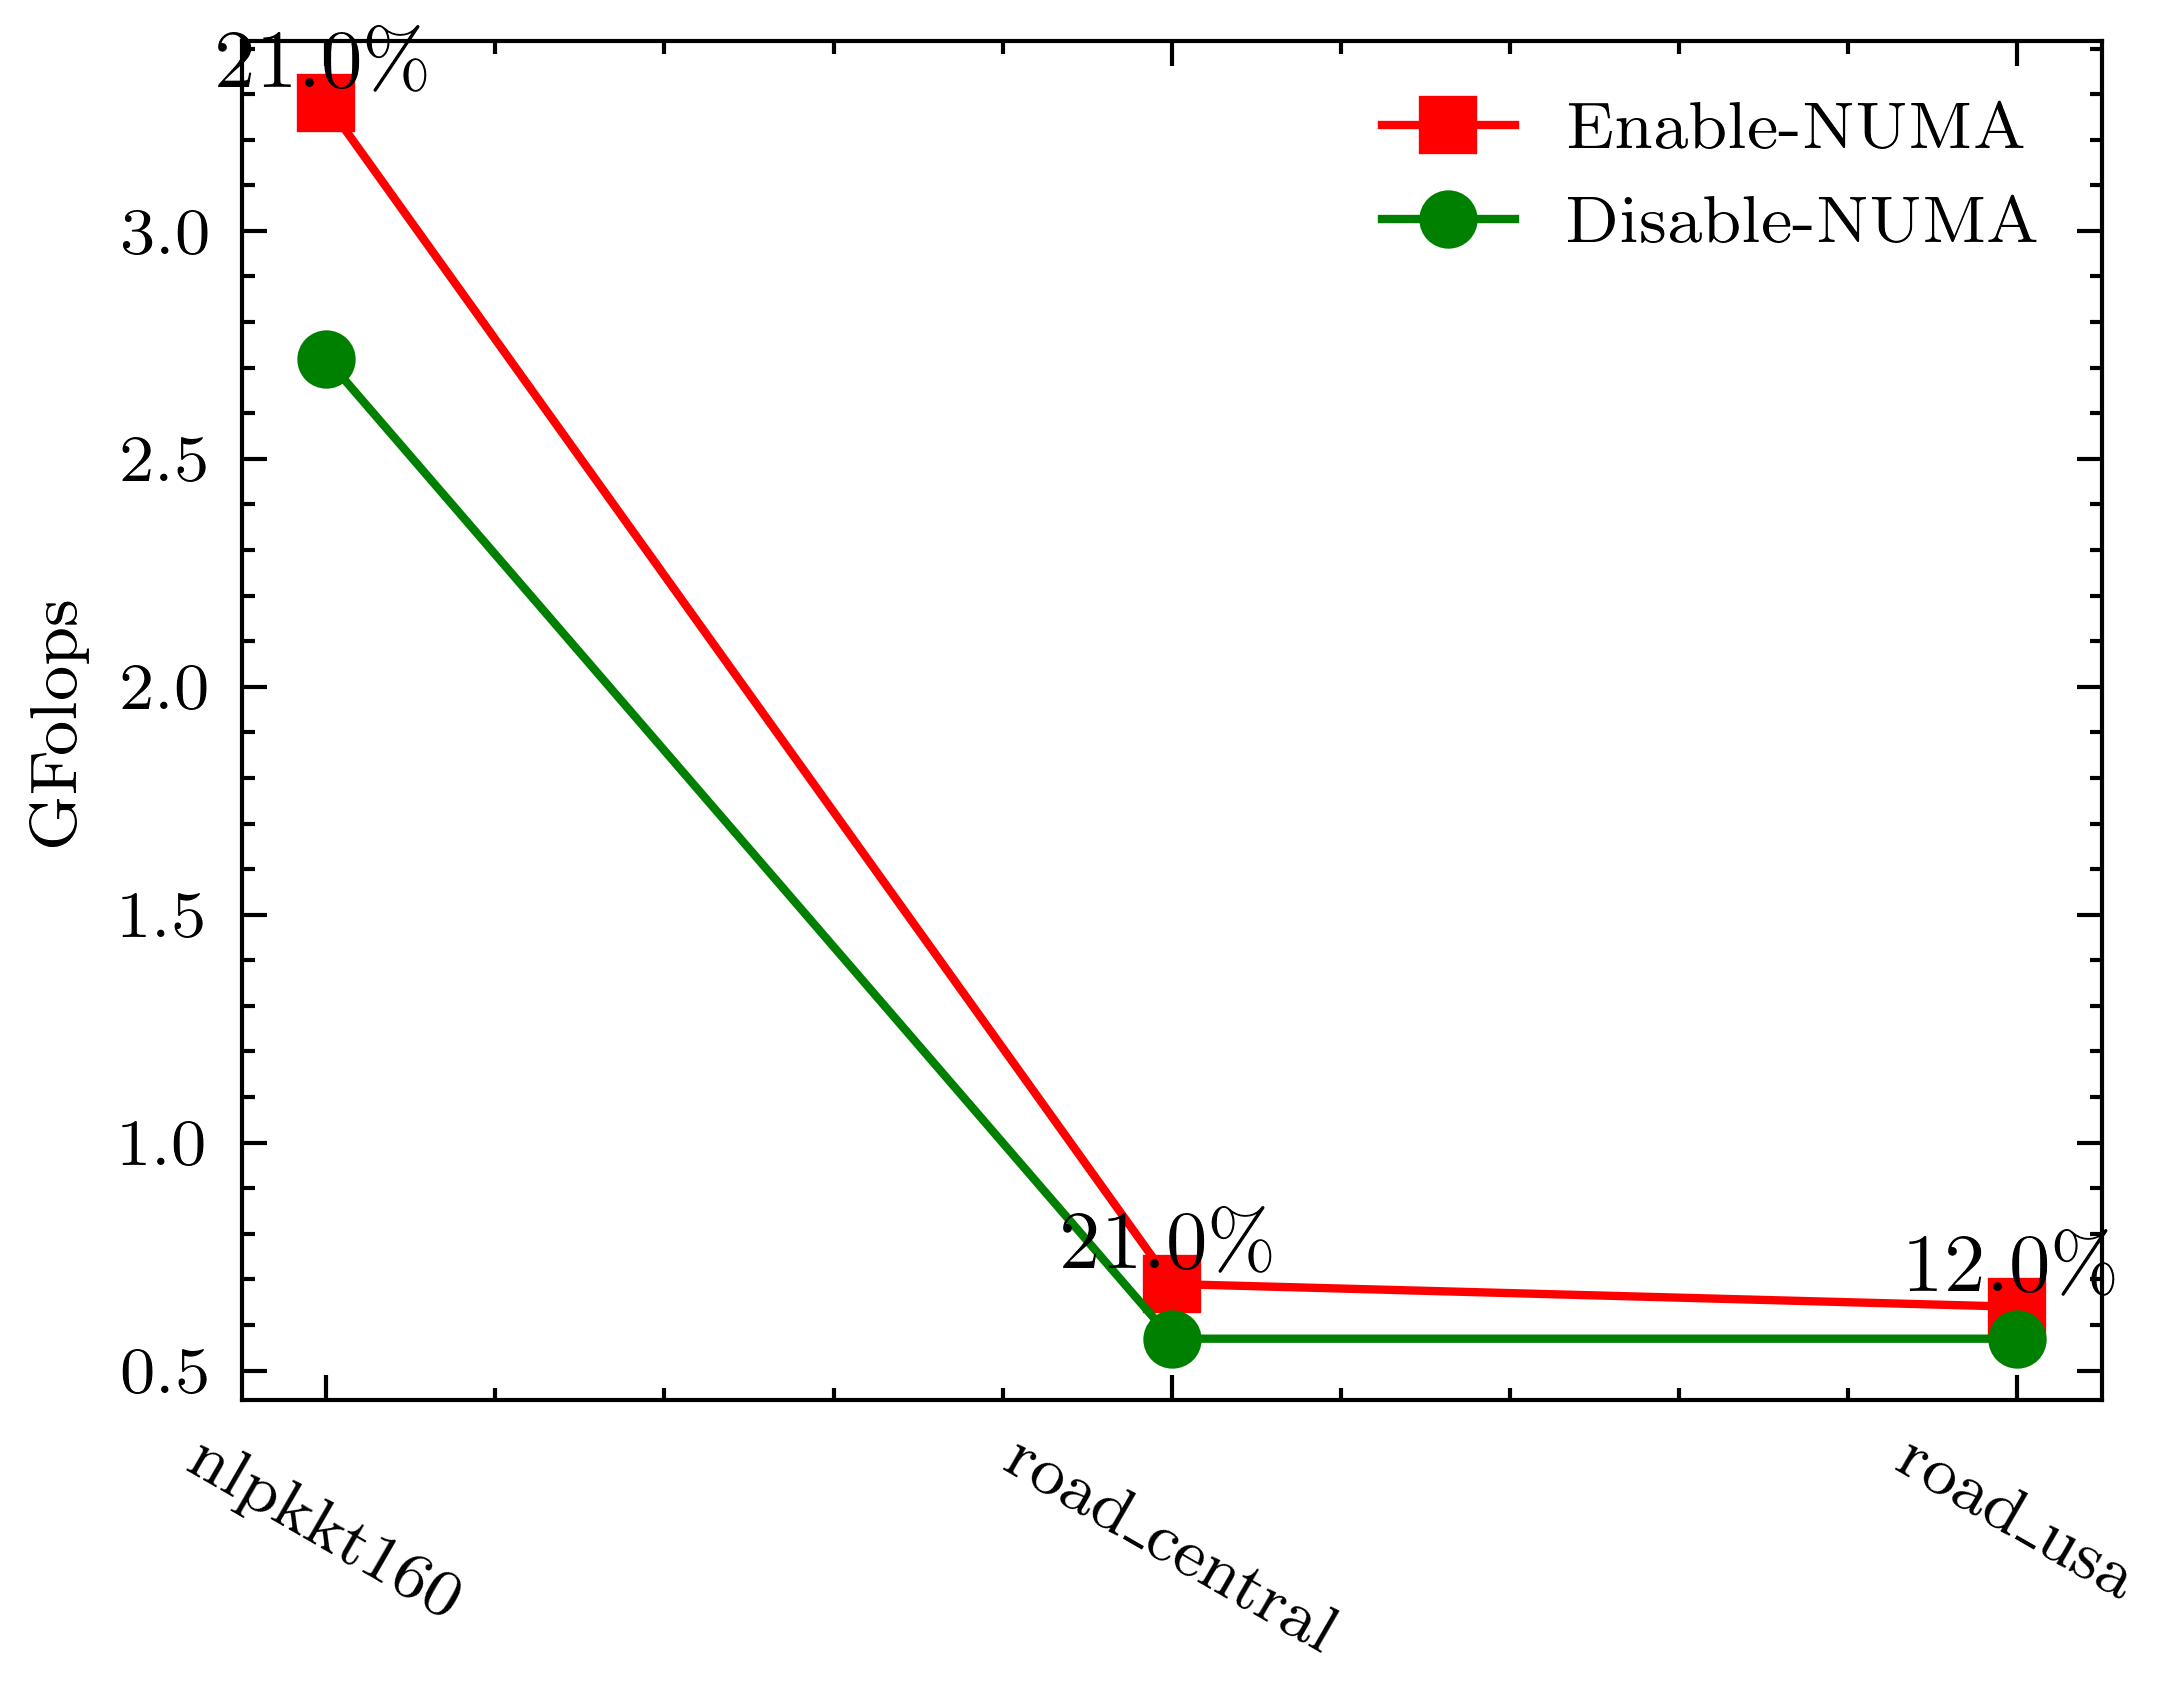
\includegraphics[width=0.7\textwidth]{NUMATEST.png}
    \caption{测试NUMA架构对性能的影响}
    \label{测试NUMA架构对性能的影响}
\end{figure}

如图\ref{测试NUMA架构对性能的影响},将cscRowPtr[]、cscColIdx[]、cscVal[]、b[],以只读数据副本的形式分配到两个NUMA结点并启用两个NUMA结点的核心之后,nlpkkt160、road\_central、road\_usa这三个规模较大的稀疏矩阵能够分别获得约21\%、21\%以及12\%的加速比。

对于规模较小或者并行性较低的矩阵,仅仅只用一个结点运行,性能更好,对于规模较大的矩阵使用多个NUMA节点进行运算能够获得更好的性能。

\section{本章总结}

本章测试分析了本文提出的SpTRSV算法的性能,并与其他平台现有的SpTRSV算法性能进行了对比,见图\ref{MatrixSuite}。同时也测试分析了算法在预处理阶段和计算阶段分别占用的时间,见表\ref{算法耗时分解表},相比于基于level-sets的算法,本文提出的SpTRSV算法的预处理时间大大减少。最后说明了本文所使用的几个优化技巧对性能的提升效果,例如使用负载均衡优化能够获得约平均23\%的性能提升、使用ARM原子指令和CPU松弛优化后一共能够获得平均10.5\%左右的性能提升、对于大规模稀疏矩阵使用NUMA架构的优化,能够获得平均约18\%的性能提升。


\endinput
\chapter{总结与展望}


\section{工作总结}

SpTRSV稀疏下三角矩阵求解是现代数值计算中的一个重要算法。是现代科学计算中一个广泛使用的计算核心,在数值模拟计算中,通常会使用迭代法或直接法求解大规模稀疏线性方程组,而SpTRSV的效率直接影响了线性方程组的求解效率,提高SpTRSV算法的性能至关重要。SpTRSV频繁且离散地数据访存、任务之间存在着很强的依赖、需要细粒度的同步、任务之间负载不均衡等特点是并行优化更加难以进行。

TODO:



\section{未来工作展望}

对于SpTRSV算法还有很多可以尝试的优化思路,例如:在任务调度方面,基于手动创建的线程池,并设计一种调度器,通过这个调度器,在线程任务分发即阶段实现任务负载均衡的操作,减少预处理的时间。并且基于这个调度器,通过一定的调度策略减少CPU自旋等待的时间,这个思路来自于GPU的硬件调度器;在访存的优化方面,目前较多的操作需要离散且频繁的从内存进行读取,导致了内存瓶颈。

\endinput

% 参考文献设置
\clearpage
\phantomsection
\addcontentsline{toc}{chapter}{\fHei 参考文献}
\sWuhao

% npu专用
\bibliographystyle{settings/nputhesis}

% 参考文献位置
\bibliography{references/reference}

% 附录
\backmatter
\input{appendix/appendix.tex}
\renewcommand{\baselinestretch}{1.5}
\fontsize{12pt}{13pt}\selectfont
\phantomsection
\chapter*{致谢}
\addcontentsline{toc}{chapter}{\fHei 致谢}

感谢党和国家

感谢老师对我的指导和帮助

感谢中科院软件研究所和华为提供的计算资源

\clearpage
\endinput
\phantomsection
\chapter*{毕业设计小结}
\addcontentsline{toc}{chapter}{\fHei 毕业设计小结}

本次毕业设计是大学阶段的最后一次挑战。期间想了很多优化的方法和思路,但是由于自身对问题认识的不够深刻,提出了一些不切实际的优化思路,并且在这些不靠谱的想法上浪费了很多时间,其中包括企图通过超图分割算法进行任务图的分割,然后绑定到NUMA结点上,来提升内存的带宽,减少总线的冲突,后来经过实践,被证实是低效的。后来我有发现了一个名为taskflow的计算框架,可以在运行时构建任务依赖图,并且使用work stealing调度算法进行并行地执行这张图,性能好于tpp和clik,但是基于该框架实现了SpTRSV算法之后,效果不是很理想。

虽然这次毕业设计对我来说是一次艰巨的挑战,但是也意义非凡。通过这次毕业设计我学习与回顾了本科所学的计算机知识,主要包括计算机组成原理和体系结构、计算机操作系统、编译原理,并将这些知识应用于实践当中,期间有想法不成功、遇到bug时候的挫败感,也有通过自己不断研究、不断实践,逐渐提升算法性能时的成就感。同时这次毕业设计也让我学到了一些科研的基础技能,为应对未来的挑战打下了基础。

总的来说,这次毕业设计是我从一个学习模仿者转变为一个创新研究者所必须经历的机遇与挑战。


\clearpage
\endinput

\clearpage
\end{document}
